% Options for packages loaded elsewhere
\PassOptionsToPackage{unicode}{hyperref}
\PassOptionsToPackage{hyphens}{url}
\documentclass[
]{article}
\usepackage{xcolor}
\usepackage[margin=1in]{geometry}
\usepackage{amsmath,amssymb}
\setcounter{secnumdepth}{-\maxdimen} % remove section numbering
\usepackage{iftex}
\ifPDFTeX
  \usepackage[T1]{fontenc}
  \usepackage[utf8]{inputenc}
  \usepackage{textcomp} % provide euro and other symbols
\else % if luatex or xetex
  \usepackage{unicode-math} % this also loads fontspec
  \defaultfontfeatures{Scale=MatchLowercase}
  \defaultfontfeatures[\rmfamily]{Ligatures=TeX,Scale=1}
\fi
\usepackage{lmodern}
\ifPDFTeX\else
  % xetex/luatex font selection
\fi
% Use upquote if available, for straight quotes in verbatim environments
\IfFileExists{upquote.sty}{\usepackage{upquote}}{}
\IfFileExists{microtype.sty}{% use microtype if available
  \usepackage[]{microtype}
  \UseMicrotypeSet[protrusion]{basicmath} % disable protrusion for tt fonts
}{}
\makeatletter
\@ifundefined{KOMAClassName}{% if non-KOMA class
  \IfFileExists{parskip.sty}{%
    \usepackage{parskip}
  }{% else
    \setlength{\parindent}{0pt}
    \setlength{\parskip}{6pt plus 2pt minus 1pt}}
}{% if KOMA class
  \KOMAoptions{parskip=half}}
\makeatother
\usepackage{longtable,booktabs,array}
\usepackage{calc} % for calculating minipage widths
% Correct order of tables after \paragraph or \subparagraph
\usepackage{etoolbox}
\makeatletter
\patchcmd\longtable{\par}{\if@noskipsec\mbox{}\fi\par}{}{}
\makeatother
% Allow footnotes in longtable head/foot
\IfFileExists{footnotehyper.sty}{\usepackage{footnotehyper}}{\usepackage{footnote}}
\makesavenoteenv{longtable}
\usepackage{graphicx}
\makeatletter
\newsavebox\pandoc@box
\newcommand*\pandocbounded[1]{% scales image to fit in text height/width
  \sbox\pandoc@box{#1}%
  \Gscale@div\@tempa{\textheight}{\dimexpr\ht\pandoc@box+\dp\pandoc@box\relax}%
  \Gscale@div\@tempb{\linewidth}{\wd\pandoc@box}%
  \ifdim\@tempb\p@<\@tempa\p@\let\@tempa\@tempb\fi% select the smaller of both
  \ifdim\@tempa\p@<\p@\scalebox{\@tempa}{\usebox\pandoc@box}%
  \else\usebox{\pandoc@box}%
  \fi%
}
% Set default figure placement to htbp
\def\fps@figure{htbp}
\makeatother
\setlength{\emergencystretch}{3em} % prevent overfull lines
\providecommand{\tightlist}{%
  \setlength{\itemsep}{0pt}\setlength{\parskip}{0pt}}
\usepackage[most]{tcolorbox}
\usepackage{chngcntr}
\newcounter{chapter}
\setcounter{chapter}{1}
\counterwithin{table}{chapter}
\usepackage{booktabs}
\usepackage{longtable}
\usepackage{array}
\usepackage{multirow}
\usepackage{wrapfig}
\usepackage{float}
\usepackage{colortbl}
\usepackage{pdflscape}
\usepackage{tabu}
\usepackage{threeparttable}
\usepackage{threeparttablex}
\usepackage[normalem]{ulem}
\usepackage{makecell}
\usepackage{xcolor}
\usepackage{bookmark}
\IfFileExists{xurl.sty}{\usepackage{xurl}}{} % add URL line breaks if available
\urlstyle{same}
\hypersetup{
  pdftitle={Chapter 1: Counting Words in the 19th-Century British Parliamentary Debates},
  hidelinks,
  pdfcreator={LaTeX via pandoc}}

\title{Chapter 1: Counting Words in the 19th-Century British
Parliamentary Debates}
\author{}
\date{\vspace{-2.5em}}

\begin{document}
\maketitle

The introduction to text mining in this book begins with tracking words'
context by processing data, counting words, and visualizing the words
that co-occur with one-another. As the linguist John Rupert Firth (1974)
said, ``You shall know a word by the company it keeps.'' Tracking subtle
variations in the context with which different words are used helps
historians and other analysts to understand the cultural biases that
structure our collective thinking. They may help us to understand how a
culture understands men and women differently, how a culture describes
people of different nationalities, the difference between a concept like
``the foreign'' and its near synonyms like ``outsider'' that
nevertheless are used in important and different ways, or how these
concepts are changing over time. In the course of this book, we will
offer a taste of the subtle and refined approaches that analysts have
used to unpack the context of different words.

Understanding the historical context of language begins with how we
interpret and approach individual words. In this chapter, we treat the
words we process as ``keywords''--terms that are central to
understanding culture and society, but whose meanings are often
contested or have shifted over time (Williams 1985). For example, the
word ``labour'' may be a particularly interesting word to an analyst of
19th-century Britain, more so than the word ``table.'' This is because
in the 19th-century debates, the meaning of the word ``labour'' evolved
alongside industrialization, class conflict, and political reform. Early
in the century, labour was often used in economic terms, referring to
the input of human work in production, as discussed by political
economists like Adam Smith. But as the century progressed---and
especially with the rise of trade unions, Chartism, and later the Labour
movement---the term labour took on a more political and moral dimension.
It began to signify not just work, but the working class itself, with
connotations of exploitation, rights, and collective struggle. The
meaning of the word ``table'' on the other hand, is generally stable,
literal, and uncontroversial. It refers to a physical object--typically
a piece of furniture--and does not carry the kind of cultural
significance that keywords do.

Recognizing words as evolving and changing--rather than fixed--allows us
to glean greater insight into how language reflects broader cultural
transformations. It invites us not to take words at face value, but to
remember that language is dynamic and often shaped by power struggles,
and that the way we process data impacts our subsequent analyses of
these power struggles.

The data processing techniques we foreground will lead to our first
visualization, where we transform individual utterances or debates into
high-level visualizations depicting the frequencies of keywords and
their associations (Moretti 2013, Jockers 2013). To achieve this end, we
will introduce three basic techniques for processing text. We will: a)
access data for the British parliamentary debates of the House of Lords
and House of Commons, 1850-59 using the \texttt{hansardr} library, b)
filter a relevant decade for keywords of interest, and c) count the
words that appear in the same context as our keywords in order to study
the associations of the keywords in more detail.

Importantly, the techniques presented in this chapter have both promise
and limits. As our companion volume, \emph{The Dangerous Art of Text
Mining} (2023), makes clear, simple word counts are almost never
sufficient on their own to support an in-depth analysis of culture.
Nevertheless, knowing how to count words and compare the context with
which different concepts are used is a first step to using text as data.
Recognizing that langauge contains keywords that can, for example, be
chosen by an analyst to guide data processing is a first step towards
producing meaning from text data.

\subsection{R Versions}\label{r-versions}

Before we get started, we need to make sure we have an up-to-date
version of R installed in order to use the packages and functions in
this book.

To check which version of R is currently running on your computer, run:

\begin{verbatim}
## [1] "R version 4.5.1 (2025-06-13 ucrt)"
\end{verbatim}

If your version is more than one major release behind (e.g., anything
below 4.3 while the current version is 4.4), you should update R from:

\url{https://cran.r-project.org}

Keeping R up to date helps ensure that your code runs
smoothly---especially when installing or loading packages, which often
require the latest versions of R to work correctly.

\subsection{Running a Line of Code}\label{running-a-line-of-code}

The first step in learning R is understanding how to run a line of code.

Here are some exercises to learn how to run code on your computer. Try
each and decide which ones feel most comfortable to you: - You can type
a command directly into the Console pane and press Enter. - You can
write it in an R script and execute it by placing your curser on the
line you want to run and press \texttt{Ctrl\ +\ Enter} on Windows or
Linux (or \texttt{Cmd\ +\ Enter} on a Mac). - You can also highlight one
or more lines of code and click the green Run button at the top of the
script editor.

Try to run the code now by typing the following into your Console and
pressing Enter, or by highlighting it and clicking Run:

\begin{verbatim}
## [1] "Hello World"
\end{verbatim}

This should display the phrase ``Hello World'' beneath your code,
confirming that R executed the command.

\subsection{Loading the Hansard Data}\label{loading-the-hansard-data}

First we will load the data we wish to analyze. Analysts, programmers,
researchers, and the like routinely import software packages developed
by others to expand the range of tools available to them.

The authors developed a data package to go with this book,
\texttt{hansardr}, to give readers an ability to access the Hansard
19th-Century British Parliamentary Debates within the R environment
(Buongiorno 2022). This is a cleaned, analysis-ready corpus of the
19th-century British Parliamentary Debates (1803-1899), also known as
``Hansard'' in reference to Thomas Curzon Hansard, the publisher. It
identifies debates whose records are missing from UK Parliament's
corpus, and it also offers a field for disambiguated speakers. We
believe this dataset will enable researchers to analyze the Hansard
debates, including speaker discourse, in a way that has not been
accessible before. Once installed, the data can be loaded with the
\texttt{data()} function.

R also has a large ecosystem of libraries---which are bundles of
additional functions, example data, and notes created by the wider R
community. Think of libraries as add-ons that expand what R can do. If
base R is the core toolkit, libraries contain all the specialty tools
others have built for tasks like text analysis, mapping, visualization,
or cleaning messy historical data.

To load these specialty tools, we use \texttt{library()}, like this.
Loading only works after the package has been installed---something we
walk through in the ``Computer Specifications and Setup'' section.

\texttt{hansardr} is now ready for use. It is conventional to load the
software packages that will be use at the beginning of each new session.
However, for the sake of demonstrating computational historical
thinking, we will regularly load packages throughout a chapter so the
reader can more easily see which functions relate back to different
packages.

When working with functions in R, it is important to remember that code
must be run in order, because each step often depends on what came
before it. For example, if we plan to use a package such as
\texttt{hansardr}, we must first load it with \texttt{library(hansardr)}
before calling any of its functions. If we skip this step, R will not
know where the \texttt{hansardr} functions come from and will return an
error such as ``could not find function,'' even if the code is correct.
Similar errors can also occur when data is not processed in the proper
sequence, since later steps may rely on datasets or data transformations
that have not yet been created.

\subsection{\texorpdfstring{Navigating the \texttt{hansardr}
Data}{Navigating the hansardr Data}}\label{navigating-the-hansardr-data}

To make working with the Hansard corpus quicker and easier--and to
prevent our personal computers from being overloaded with too much data
at once--we partitioned the century long corpus into decade sections. In
the field of data analysis, it is common to call these sections
``subsets.''

The first subset we will meet is a collection of the speeches of
parliament, 1850-59, broken into sentences, where each row of the data
frame is one sentence. Later, we will meet more datasets that contain
``metadata,'' or information about the speaker, year and date of the
speech, and other important contextual information for historical
analysis.

The \texttt{hansardr} corpus is subsetted by decade. As shown by Table
1, each decade has four types of data, labeled: \texttt{hansard},
\texttt{debate\_metadata}, \texttt{speaker\_metadata}, and
\texttt{file\_metadata}. In the following table, ``YYYY'' stands in for
any given decade.

\begin{longtable}[]{@{}
  >{\raggedright\arraybackslash}p{(\linewidth - 4\tabcolsep) * \real{0.2821}}
  >{\raggedright\arraybackslash}p{(\linewidth - 4\tabcolsep) * \real{0.5641}}
  >{\raggedright\arraybackslash}p{(\linewidth - 4\tabcolsep) * \real{0.1538}}@{}}
\caption{Overview of the hansardr corpus, showing the primary text files
and their associated metadata. Each data set is linked through a common
sentence ID.}\tabularnewline
\toprule\noalign{}
\begin{minipage}[b]{\linewidth}\raggedright
Label
\end{minipage} & \begin{minipage}[b]{\linewidth}\raggedright
Description
\end{minipage} & \begin{minipage}[b]{\linewidth}\raggedright
Key
\end{minipage} \\
\midrule\noalign{}
\endfirsthead
\toprule\noalign{}
\begin{minipage}[b]{\linewidth}\raggedright
Label
\end{minipage} & \begin{minipage}[b]{\linewidth}\raggedright
Description
\end{minipage} & \begin{minipage}[b]{\linewidth}\raggedright
Key
\end{minipage} \\
\midrule\noalign{}
\endhead
\bottomrule\noalign{}
\endlastfoot
hansard\_YYYY & Hansard debate text & sentence\_id \\
debate\_metadata\_YYYY & Metadata such as speech date and title. &
sentence\_id \\
speaker\_metadata\_YYYY & Metadata on speakers. & sentence\_id \\
file\_metadata\_YYYY & Metadata for source file, column, and more. &
sentence\_id \\
\end{longtable}

Both text and metadata are divided into subsets named by decade, for
instance, \texttt{hansard\_1850}. \texttt{hansard\_1850} contains just
the speech text as well as a unique sentence ID that can be used to
connect the speech text with its corresponding metadata. We will
demonstrate this process later in \emph{Text Mining for Historical
Analysis}.

Processing both text and dates is important for historical analysis. In
this chapter, we will start working exclusively with text--not
dates--because they are easy to process when counting words. But the
other subsets within \texttt{hansardr} contain other data types.

We can use \texttt{data()} to load one of these decade-based subsets of
the Hansard corpus.

A new variable named \texttt{hansard\_1850} is now able to be seen in
our Global Environment panel. If you are using RStudio, you can explore
the data by clicking on its name in the Global Environment pane (the top
right quadrant of RStudio). Clicking on the name of the dataset will
open a new tab containing a view of the data, which can be searched for
a keyword, like in a spreadsheet. One can also double-click on any row
in the data frame to select a row, then copy that data and paste it into
a Word Document or other tool.

The Hansard subsets are purposefully small enough to open and explore on
a personal computer. When working with larger datasets, it may not be
possible to open the entire dataset in another tab. Instead, in the
Global Environment Panel you can also click on the blue
``\textgreater{}'' symbol to the left of each data frame to display the
``fields'' by which the dataset is structured, in this case, the names
of the columns in the dataset, as well as a preview of the content of
each of these columns.

In addition to exploring the data in RStudio, there are a few functions
that provide the means to look at sections of the dataset in greater
detail. Throughout this book, we will routinely ``inspect'' the data by
using functions like \texttt{head()} to see how the data is transformed
at different processing steps. Getting into the habit of using functions
like \texttt{head()} makes it easier to notice and interrogate problems
as they arise, or ensure that the data transformations meet
expectations. At the console, an analyst can also use \texttt{head()} to
ask R to display the first six rows of the data. In some versions of
RStudio you will see an arrow that allows you to move between two
columns.

As shown by Table 2, the first column in this dataset is
\texttt{sentence\_id}, which gives a unique identifier for each
sentence, including information about which series of parliamentary
proceedings we are looking at, which volume and page, and which sentence
number on each page. The second column is \texttt{text}. Each row is a
distinct sentence of text. These speeches were broken into sentences
during the dataset creation stage, where the authors wrote a script to
detect punctuation and line breaks.

Below is an excerpt from \texttt{hansardr}:

\begin{table}
\centering
\caption{\label{tab:hansard_corpus_sentence_text}Excerpt from the 1850 Hansard corpus showing 
                 sentence-level text with associated sentence ID values.}
\centering
\resizebox{\ifdim\width>\linewidth\linewidth\else\width\fi}{!}{
\begin{tabular}[t]{lp{12cm}}
\toprule
sentence\_id & text\\
\midrule
S3V0108P0\_0 & , which had been prorogued successively from the 1st of August to the 9th of October, from thence to the 20th of November, thence to the 16th of January, and from thence to the 31st January, met this day for despatch of business.\\
S3V0108P0\_1 & The Parliament was opened by Commission, the LORDS COMMISSIONERS present being the LORD CHANCELLOR; the LORD PRESIDENT OF THE COUNCIL (the Marquess of Lansdowne); the LORD PRIVY SEAL (the Earl of Minto); the LORD CHAMBERLAIN OF THE HOUSEHOLD (the Marquess of Breadalbane); and the LORD BISHOP OF LONDON.\\
S3V0108P0\_2 & called attention to a great omission of their duty on the part of Ministers, with respect to the privileges of their Lordships, which might and ought to have been avoided.\\
S3V0108P0\_3 & At pre-sent there were two vacancies in the representative Peers of Scotland, in consequence of the deaths of the Earl of Airlie and of Lord Colville.\\
S3V0108P0\_4 & Although the Act of Parliament directed that the proclamation should issue forthwith for the election of representative Peers to fill up any vacancies which might occur, by death or otherwise, no such proclamation had yet taken place in the case of the two vacancies he had just mentioned, and the consequence was, that for twenty-four days after the meeting of Parliament it was not possible for any Scotch representative Peers to be elected.\\
\bottomrule
\end{tabular}}
\end{table}

To display the data in a more visually appealing format, we can use the
\texttt{knitr} package, which provides the \texttt{kable()} function for
creating clean, basic tables from R objects. We then enhance these
tables with the \texttt{kableExtra} package, which adds styling
options---such as custom column widths, captions, alignment, and
shading---allowing us to produce polished, publication-quality tables.

\subsection{Tidy Text Mining and Loading
Libraries}\label{tidy-text-mining-and-loading-libraries}

Most of the functions used in the first chapters of this book come from
a software package called \texttt{tidyverse} (2019) which is a family of
smaller packages developed by Chief Scientist at Posit (formerly known
as RStudio), Hadley Wickham. The \texttt{tidyverse} was created to order
data in ``tidy'' tables where it is structured as a data frame made up
of columns and rows. In other words, the \texttt{tidyverse} is built to
work with data like \texttt{hansard\_1850}.

We have found that a tidy approach to text exploration and analysis
allows us to write code quickly and effectively, giving us ample control
over the data and allowing us to inspect the output of every data
processing step and type of analysis. This library thus supports
analysts focusing on questions about data processing and history without
being weighed down by the nuances of different structural and syntactic
coding problems.

We distinguish between writing code and processing data, proposing that
data processing and historical analysis are co-creative practices. Data
processing shapes how we interpret the past---it is not a neutral task,
but one that governs the possibilities of historical understanding. At
the same time, the historical material we study--the observations we
make--might inform and reshape our data processing methods. We will
return to this central idea of ``computational historical
thinking''--which we introduce in our introduction--throughout the book,
as we demonstrate how iterative adjustments to our processing approach
impact our analysis.

In this chapter we will also use the \texttt{tidytext} library,
developed by David Robinson and Julia Silge (2016), to work with textual
data. The \texttt{tidytext} library contains a variety of tools useful
for processing text and treating text as data. Many sections in this
book will therefore begin by loading the two libraries
\texttt{tidyverse} and \texttt{tidytext}.

\subsection{Using Functions to Process
Data}\label{using-functions-to-process-data}

The primary purpose of a function is to create reusable code, allowing
analysts to avoid repeating the same data processing steps over and
over.

From this point on we are going to use more complicated functions from
different R packages to process our data. Before we take this next step,
however, we first want to provide a basic understanding of a function's
underlying components, by creating our own simple function:

The above code can be broken down into these core parts:

\begin{enumerate}
\def\labelenumi{\arabic{enumi}.}
\tightlist
\item
  Function Name: The name given to the function. In this example, the
  function is named \texttt{add\_numbers}.
\item
  Parameters: The variables listed in the function definition that will
  accept arguments, for instance, \texttt{function(a,\ b)}.
\item
  Body: The code that is executed when the function is called, written
  here as \texttt{result\ \textless{}-\ a\ +\ b}.
\item
  Return Value: The output produced by the function, for example,
  \texttt{return(result)}.
\end{enumerate}

Every function in R encapsulates a code body, even when it is hidden
from the analyst.

We can now use our new \texttt{add\_numbers()} function by passing
arguments to the specified parameters. In this example, the ``a''
parameter is passed the number 2, and the ``b'' parameter is passed the
number 3. The two numbers are added in the body, and then the results
are returned.

Now that we have defined this function, we can call upon it whenever we
need to add two numbers without rewriting the steps involved. This kind
of reuse becomes especially important in historical analysis, which is
often iterative and rarely linear. As our interpretations shift and our
questions evolve, we often return to the same operations with new
purposes. Having stable tools like functions allows us to revisit and
revise our analyses without starting from scratch each time.

\begin{verbatim}
## [1] 5
\end{verbatim}

To count words in Hansard, we will use a different function, the
\texttt{unnest\_tokens()} function from \texttt{tidytext}. While there
are many ways to count words over time, one way to do this--that is also
very human readable--is to put our data into a format where each word of
the text is on a separate row. These individual words are called
``tokens.'' The process of splitting chunks of text into individual
units is called ``tokenization.'' While singular words are often called
``tokens,'' a common term used to instead describe multi-word phrases is
``n-gram'' (such as using the term ``bigrams'' to describe sequential,
two-word phrases).

In this one-token-per-row format we can easily process our data. This
approach to data processing is common in the humanities and handles text
using the ``Bags of Words'' (BoW) approach, where text data is treated
as a collection (or ``bag'') of individual words without regard to
grammar, order, or context (Jockers 2015). The focus is instead on word
frequency or occurrence.

The above code also has new symbols, called ``operators.'' Operators are
essential for data processing. Throughout the course of this book we
will introduce multiple different kinds of operators.

The assignment operator, \texttt{\textless{}-}, sometimes translated as
``gets,'' points to the output of a function and is followed by the name
of an original dataset. The \texttt{\%\textgreater{}\%} operator, called
a ``pipe,'' and translated as ``next,'' is used to chain together
successive transformations of a dataset. This will make more sense when
we cover more examples later in the book.

If this is your first time using a programming language for analysis, it
can be useful to practice reading each line of code as a sentence of
instructions that tells the computer what output to make, what input to
use, and what processes to go through in a certain order. We sometimes
suggest that first time programmers translate code into a series of
English sentences, using their knowledge of the \texttt{\textless{}-}
and \texttt{\%\textgreater{}\%} operators, the names of variables, and
their understanding of distinct commands. The code above be read as
follows: ``Create a new variable called \texttt{tokenized\_hansard}.
Start with the dataset \texttt{hansard\_1850}. Next, unnest the tokens
in the''text'' column of \texttt{hansard\_1850}, unpacking those strings
of text into individual words.''

One may also notice the arguments passed to \texttt{unnest\_tokens()},
``word'' and ``text.'' Functions like \texttt{unnest\_tokens()} take a
set number of arguments, typically in a precise order. The first
argument is the type of unnesting that will be employed. The second
argument is the name of the column from the original
\texttt{hansard\_1850} data that we will work on, in this case,
``text.''

As you inspect the arguments of each function, consider the fact that
those arguments exist because they allow the analyst to change the
arguments to get different results. With the \texttt{unnest\_tokens()}
function, the analyst could hypothetically choose to ``unnest'' the
sentences into tokens of different length, for instance, sentences,
n-grams, or other units of text. In later chapters we will explore some
of these capabilities of the \texttt{unnest\_tokens()} function.
Alternatively, if \texttt{unnest\_tokens()} were being applied to a
different dataset where the column had a different name than ``text,''
we could change the column name from ``text'' to something else. In
later examples, we will use the same commands applied to different
datasets with different column names. For now, we will mainly use
\texttt{unnest\_tokens()} with the arguments ``word'' and ``text.''

Next, let's inspect the results of our unnesting using \texttt{head()},
which returns just the first rows of a data frame.

\begin{verbatim}
##   sentence_id         word
## 1 S3V0108P0_0        which
## 2 S3V0108P0_0          had
## 3 S3V0108P0_0         been
## 4 S3V0108P0_0    prorogued
## 5 S3V0108P0_0 successively
## 6 S3V0108P0_0         from
\end{verbatim}

However, we have a preference for looking at more data since that can
give us a fuller picture of the data.

\begin{verbatim}
##    sentence_id         word
## 1  S3V0108P0_0        which
## 2  S3V0108P0_0          had
## 3  S3V0108P0_0         been
## 4  S3V0108P0_0    prorogued
## 5  S3V0108P0_0 successively
## 6  S3V0108P0_0         from
## 7  S3V0108P0_0          the
## 8  S3V0108P0_0          1st
## 9  S3V0108P0_0           of
## 10 S3V0108P0_0       august
## 11 S3V0108P0_0           to
## 12 S3V0108P0_0          the
## 13 S3V0108P0_0          9th
## 14 S3V0108P0_0           of
## 15 S3V0108P0_0      october
\end{verbatim}

\texttt{unnest\_tokens()} did a lot of heavy lifting for us!

As part of our data transformation, the output data has a column named
``word'' for each individual token of the corpus. Notice that the words
in \texttt{tokenized\_hansard} look just like the words in the first
sentence of the first speech in \texttt{hansard\_1850}. Those speeches
have been split into individual words, but the words are still in the
same order. Notice that the command \texttt{unnest\_tokens()} has also
transformed all the words to lower-case and removed punctuation marks
such as commas and periods. This transformation, often called ``data
cleaning'' will make the words easier to count because the computer will
not treat words differently based on capitalization or the presence of
symbols.

As we inspect the results of unnesting, one might note that the input to
\texttt{unnest\_tokens()} was ``tidy'' in format -- that is, it had two
columns, one for ``sentence\_id'' and one for ``text''. After working
with \texttt{unnest\_tokens()}, the resulting output,
\texttt{tokenized\_hansard}, also is ``tidy'' in format. That is, it has
two columns, one for \texttt{sentence\_id} and one for \texttt{word}.
This tidy format is both easily human readable and also easy to process
and count.

\subsection{Counting Words}\label{counting-words}

Now we are going to bring together what we have learned by chaining
together multiple functions that will be used to process the Hansard
data.

The \texttt{count()} function from the \texttt{tidyverse} groups like
tokens with like tokens, then counts them. Below, we are passing
\texttt{count()} one argument, the name of the column to operate on--in
this case, ``word'' from the tokenized hansard data.

\begin{verbatim}
##   word       n
## 1  the 2588864
## 2   of 1404831
## 3   to 1126226
## 4 that  726686
## 5  and  706117
## 6   in  597753
\end{verbatim}

With the command \texttt{arrange(desc(n))}, we tell the computer to
arrange the results from greatest to least. We perform this step so that
the results are easier to read, not because this step is necessary for
counting words.

We now have a frequency count of every word recorded in the speeches of
Hansard, 1850-59. The initial results are unimpressive. In our dataset,
as with most textual datasets, the most common words are also often the
least interesting. For this reason, analysts compile lists of the most
common words, called ``stop words.'' Analysts often remove stop words
from their results before analysis.

The \texttt{tidytext} package comes with a prepared list of stop words.
We can remove them from our results by loading the ``stop\_words''
dataset and then passing the dataset as an argument to the
\texttt{anti\_join()} function. \texttt{anti\_join()} keeps all the rows
in the first dataset that do not have a match in the second dataset.
Using \texttt{anti\_join()} we can remove words we do not want in our
analysis from our data.

\begin{verbatim}
##         word      n
## 1        hon 125465
## 2      house 118861
## 3 government  95417
## 4       bill  77322
## 5      noble  73180
## 6       lord  68942
\end{verbatim}

These results cleaned of their stop words seem sensible for parliament.
Some of them demonstrate the way that members of parliamentarians refer
to each other, for example, as ``my noble lord'' or ``the
hon{[}ourable{]} member {[}in question{]}.'' Speakers in parliament also
routinely refer to the business of parliament, especially referencing
the ``house {[}of commons or lords{]},'' the ``bill'' or ``question''
under debate, the state of the ``country,'' and how much ``time'' is
available for debate.

General words, of course, give us little insight into the business of
parliament. Later sections will give us richer tools for examining how
the content of speeches changed over time. For now, we have successfully
achieved the first step of analysis, the processing of text into words,
and the counting of words.

\subsection{Searching for Keywords}\label{searching-for-keywords}

The \texttt{tidyverse} package provides several commands that we will
use throughout this book to track individual keywords. The
\texttt{filter()} function allows us to find an exact match within the
data. Suppose that we want to inspect the tenth sentence of the
parliamentary speeches, series 3, volume 108, which has the id number
``S3V0108P0\_10.'' Alternately, \texttt{filter()} can be used to subset
the \texttt{stopworded\_hansard\_counts} data frame, returning only the
rows where the word column contains the value ``india''.

\begin{verbatim}
##    word     n
## 1 india 20816
\end{verbatim}

In this code, we pass \texttt{filter()} two arguments: first, the name
of the column we will search for (``word''), and second the name to
match (``india''). Here we are using the \texttt{==} operator to
indicate we want to return an exact match, as opposed to returning words
that might contain the word ``india'' such as ``indian''.

We can do the same for any other keyword of interest.

\begin{verbatim}
##     word    n
## 1 france 7146
\end{verbatim}

\begin{verbatim}
##      word   n
## 1 jamaica 475
\end{verbatim}

Filtering for every word we wish to track, one-by-one, can be tedious
and time consuming. Filter can also be used with other R operators, such
as \texttt{\%in\%}, that save us time and energy by giving us the
opportunity to cycle through multiple words of interest instead of just
one.

To do this, we can first create our own custom list of words we wish to
analyze.

Now we can use the \texttt{\%in\%} operator to check if a word from our
list, \texttt{identifiers\_for\_woman}, is in the ``word'' column.

\begin{verbatim}
##           word    n
## 1         wife 2222
## 2       sister 1153
## 3        woman 1063
## 4        women 1062
## 5        wives  479
## 6        widow  315
## 7       female  294
## 8       widows  254
## 9      sisters  240
## 10     females  195
## 11       girls  180
## 12        girl   76
## 13        aunt   62
## 14 grandmother   18
## 15       aunts   10
\end{verbatim}

\texttt{filter()} is useful for more than just text data. It also works
on quantitative data with comparison operators like the greater than,
\texttt{\textgreater{}}, or less than, \texttt{\textless{}}, signs. This
is handy if we want to filter for words that are said more or less than
a specified number of times, as one example. For the sake of
readability, we are only going to show the first 20 words that follow
our filter.

\begin{verbatim}
##          word   n
## 1    contrast 473
## 2      pardon 473
## 3    thirteen 473
## 4   elizabeth 472
## 5    laboured 472
## 6       renew 472
## 7        seal 472
## 8     trustee 472
## 9          19 471
## 10    compare 471
## 11   concerns 471
## 12  denounced 471
## 13  mortality 471
## 14   publicly 471
## 15    silence 471
## 16    uttered 471
## 17      pride 470
## 18 sacrifices 470
## 19 acceptance 469
## 20    secrecy 469
\end{verbatim}

We can also use multiple operators in conjunction with one-another. In
the following code we do this by supplying the \texttt{\&} operator to
combine multiple conditions. The following example filters rows where n
is greater than 474 and less than 476.

\begin{verbatim}
##           word   n
## 1       cities 475
## 2   depositors 475
## 3      jamaica 475
## 4        pause 475
## 5       shared 475
## 6 unfavourable 475
\end{verbatim}

In just this quick glimpse of our data, meaningful words are beginning
to appear. The word ``Jamaica,'' for example, appears along with the
word ``depositors.'' These words hint at the political, economic, and
social issues of the time, specifically the declining state of the
economy. Members of Parliament discussed the slave revolt in Jamaica,
including its scale and significance. Since the 17th century, Jamaica
had its own parliament but was placed under martial law during the
revolt. Its appearance here demonstrates that Jamaica was significant
enough to command parliamentary attention, elevating the revolt to a
major historical event that could not be ignored by Parliament.

\subsection{Tailoring our Word Count
Analysis}\label{tailoring-our-word-count-analysis}

Detecting and filtering for keywords of interest can be particularly
meaningful for using data to tell history.

Our next function, \texttt{str\_detect()}, treats data as patterns and
detects their presence or absence. It returns \texttt{TRUE} if the
pattern is detected, or \texttt{FALSE} if it is not. When a data type
represents only two possible values, \texttt{TRUE} or \texttt{FALSE}, it
is typically referred to as a ``Boolean'' value.

In the following example, we iterate through each word in the
\texttt{identifiers\_for\_woman} list to check whether the value
contains ``girl.''

\begin{verbatim}
##  [1]  TRUE FALSE  TRUE FALSE FALSE FALSE FALSE FALSE FALSE FALSE FALSE FALSE
## [13] FALSE FALSE FALSE FALSE
\end{verbatim}

The results from \texttt{str\_detect()} are not very telling for
analysis. Instead, for a textual analysis we often use both functions,
\texttt{filter()} and \texttt{str\_detect()}, together so that we return
a more human-readable result.

The following example searches \texttt{hansard\_1850} for the keyword
``coal.'' Notice that \texttt{str\_detect()} is nested inside the
command \texttt{filter()}. Together, these commands tell the computer to
filter for only those rows of the column ``text'' that contain the
keyword ``coal.''

Something else interesting is happening in our code. The word ``coal''
has a funny looking set of characters,
\texttt{\textbackslash{}\textbackslash{}b}, on either side. Together
with the word ``coal,'' these special characters are make up part of a
``regular expression'' often abbreviated as ``regex.'' Regular
expressions are sequences of characters that define search patterns,
typically used for string matching, processing, and extraction.

One reason the \texttt{str\_detect()} function is so special is because,
unlike \texttt{filter()} by itself, the \texttt{str\_detect()} function
enables us to match with regular expressions, not just words.
\texttt{\textbackslash{}\textbackslash{}b} indicates a word's
boundaries. It matches the position between a word character (e.g.,
letters, numbers) and a non-word character (e.g., space, punctuation, or
the start/end of a string). \texttt{\textbackslash{}\textbackslash{}b}
at the end ensures that ``coal'' is a standalone word, meaning it will
match ``coal'' but not ``coalesce'' or ``charcoal.''

The result of our search is variable, \texttt{hansard\_coal}, that
contains only sentences from the 1850 debates that contain the word
``coal.''

\begin{longtable}{>{\raggedright\arraybackslash}p{14cm}}
\toprule
text\\
\midrule
The manufacturers of this country relied on their capital, and their command of
coal and iron, for a continuance of their prosperity; but, again, let them cast
their eyes on the other side of the Atlantic.\\
Mines, also, except coal, clay pits, slate quarries, and other descriptions even
of real property escaped the operation of the Act.\\
One class of offences which was more particularly adverted to in this part of
the Bill, was that of the offence of coal stealing.\\
A coal-owner told him that he was plundered of many tons of coal per week, owing
to the difficulty of prosecuting the offenders.\\
They were subjected to great loss by the theft of small articles of coal, and
they submitted from time to time to the injury rather than prosecute; till, at
last, they found themselves compelled to proceed against some person for the
theft of an article not amounting, perhaps, to more than a penny in value.\\
\addlinespace
Here, perhaps, is one county abounding in coal and stone—the latter advantageous
for the construction of houses for all classes.\\
\bottomrule
\end{longtable}

\subsection{Finding and Comparing Keywords'
Context}\label{finding-and-comparing-keywords-context}

Typically, we want to do more than simply search for a singular keyword.
We may also want to search for collocates, or words that are
``co-located'' next to one-another. These words form the linguistic
context of a given keyword.

We already have everything we need to make this happen: we can search
for a keyword, we can break up text into words, and we can count the
words. We can use our knowledge to search for the context of several
keywords and compare them in visual form.

The following code chains multiple data processing steps together.

Instead of running these functions independently, we have chosen to
chain them together with the pipe, \texttt{\%\textgreater{}\%},
operator. Using the pipe allows us to use many functions sequentially
without storing intermediary variables.

Notice the line of code that reads
\texttt{filter(!str\_detect(word,\ "{[}:digit:{]}"))}.
\texttt{{[}:digit:{]}} is a regular expression in R that matches all
digits, this way we do not have to specify them one-by-one. We added
\texttt{!} to filter out any entries that comprise digits. The negation
operator, \texttt{!}, tells R to do the opposite of what the function
usually does. Using it in the \texttt{filter()} function and preceding
\texttt{str\_detect()}, we ask to return text, not digits like the dates
recorded in Hansard.

\begin{verbatim}
##         word   n
## 1       coal 422
## 2      steam  50
## 3     duties  46
## 4       bill  42
## 5 government  40
## 6      mines  40
\end{verbatim}

These are the words that appear most frequently with the word ``coal.''
When sharing our results, however, we may want to visualize our data
instead of providing a table so we can analyze collocates more easily.

We can visualize just the top 20 words that co-occur with the word
``coal'' by selecting the \texttt{top\_n(20)} appearances from our
sorted data.

To visualize our data, we will use \texttt{ggplot}. \texttt{ggplot} is
an R package used for creating visualizations. It follows an approach
that allows users to build plots layer by layer, combining data,
aesthetics (e.g., axes, colors), and geometric objects (e.g., points,
lines) to create visualizations. We will use \texttt{ggplot} frequently
throughout this book.

\begin{figure}
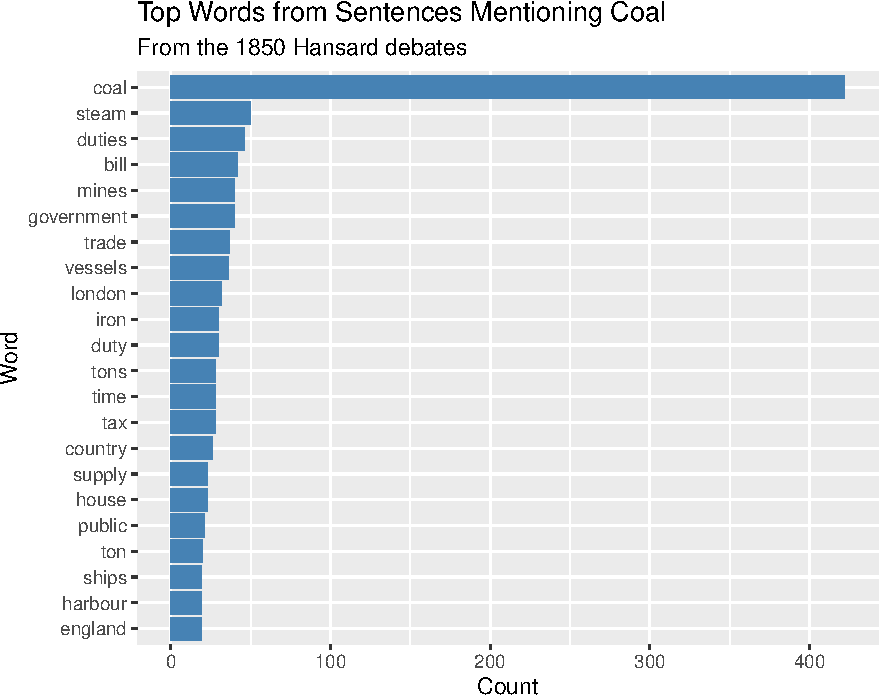
\includegraphics[width=0.8\linewidth]{ch1-11.25.2024_files/figure-latex/visualize_coal_context-1} \caption{Top words in sentences mentioning coal (Hansard, 1850)}\label{fig:visualize_coal_context}
\end{figure}

Figure 1.1 displays the results of our code: a bar chart showing how
many times ``coal'' was mentioned, along with the most frequent words
that co-occur with the term. Note that because we are analyzing
collocates, these counts do not reflect the total number of times they
were mentioned between 1850 to 1859. Instead, the counts represent the
total number of times these words appear in the same context as
``coal.''

The second most frequent word is ``steam'' followed by ``duties,''
``bill,'' and ``mines.'' Words like ``duty,'' ``iron,'' ``tax,'' and
``supply'' indicate key economic and industrial topics related to coal
during the debates, with ``iron'' possibly tied to the role of coal in
iron production. ``Harbour,'' ``ships,'' and ``vessels'' suggest
discussions related to transportation and trade of coal.

Rather than focusing on specific speeches, this method of visualizing
data allows us to trace broader semantic and thematic structures that
shaped the discourse around the keyword coal in the 1850s. By
aggregating linguistic data over time, we can detect not only the
persistence of industrial and economic concerns, but also a macroscopic
view of historical language.

Taken together, the visualization emphasizes the central role of coal in
the British economy and legislation in the 1850s, as well as its links
to other industrial and governmental matters. The visualization also
reflects concerns around infrastructure, taxation, and policy decisions
regarding coal.

Our analysis will gain nuance the more we compare near concepts. While
coal was important to powering Britain's industrial revolution, perhaps
the most controversial economic debates of the 1850s revolved around the
issue of the Corn Laws, the system of taxation of wheat and other
grains, which were originally introduced to protect British farmers.
Working-class demands for cheap bread led to the repeal of the Corn Laws
in 1846. Knowledge of these facts might lead us to ask: were coal and
corn debated using the same language or different words?

\begin{verbatim}
##      word    n
## 1    corn 2085
## 2    laws  556
## 3 country  426
## 4    duty  333
## 5   price  325
## 6  repeal  274
\end{verbatim}

Already we can see the words that most frequently co-occurred with our
keyword ``corn.'' Visualizing the top 20 words using \texttt{ggplot}
makes this context easier to apprehend.

\begin{figure}
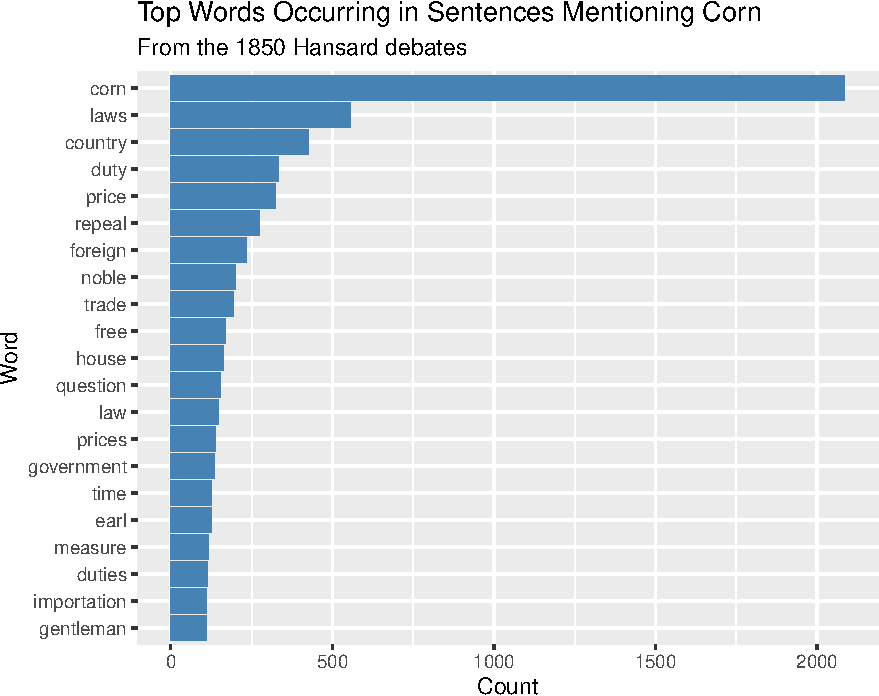
\includegraphics[width=0.8\linewidth]{ch1-11.25.2024_files/figure-latex/visualize_corn_context-1} \caption{Top words in sentences mentioning corn (Hansard, 1850)}\label{fig:visualize_corn_context}
\end{figure}

Comparison between Figure 1.1, the words used in the context of coal,
and Figure 1.2, the words used in the context of coal, gives us a
foothold for beginning to think about how taxation was discussed in
different contexts. For instance, the context of both keywords reference
the role of ``time'', ``duties'', ``taxes'', and the ``government'', but
debates over corn are more linked to the question of Britain's
dependence ``foreign'' powers, whereas debates over coal are more
crucially related to the condition of ``England'' itself.

Further research would be necessary for an analyst to decide whether
comparing these two commodities as keywords is worthwhile, and which
collocates offer insight. Nevertheless, at this point we have
demonstrated a preliminary process with which most of the analyses in
this book will start: by loading data, inspecting data, breaking that
data into words, and counting those words. Later chapters will
complicate this process, giving us more sophisticated approaches to
understanding historical change and change over time.

This foundational workflow, loading, inspecting, tokenizing, and
counting words, lays the groundwork for more nuanced textual inquiries.
One such method, which begins to address the limitations of mere
frequency counts, is the ``Keywords in Context'' (KWIC) approach.

\subsection{Finding a Word's Context using ``Keywords in Context''
(KWIC)}\label{finding-a-words-context-using-keywords-in-context-kwic}

In the 1950s, Jesuit scholar Father Roberto Busa partnered with IBM to
create a machine-readable concordance of the works of Thomas Aquinas,
known as the Corpus Thomisticum (Jones 2016). As a Jesuit scholar deeply
immersed in Thomistic philosophy, Busa wanted to analyze the use and
meaning of the Latin word ``in''---a preposition with significant
theological weight---in the complete works of Thomas Aquinas. These
texts contained over 11 million words, making it virtually impossible to
conduct such a study without first restructuring the material for
analysis. However, the challenge he faced was not only the scale of the
corpus, but the need to preserve the linguistic and philosophical nuance
of Aquinas's writings.

Widely regarded as the inception of the digital humanities, Busa's work
demonstrated the transformational potential of computing for humanistic
inquiry. Busa's project marked a pivotal shift in textual scholarship by
introducing computational methods to the humanities. By producing a
machine-readable concordance of Thomas Aquinas's works, the project laid
the foundation for techniques now central to digital textual analysis,
including the use of KWIC (Keywords in Context) displays.

Concordance-style views have remained central to the study of language
and meaning in the humanities. While collocates are one way to explore a
word's context---by analyzing frequently co-occurring tokens---they are
not the only method. Tools like ``Keywords in Context'' (KWIC),
available in the \texttt{quanteda} library, provide a concordance-style
view that presents sentence-level context. This allows researchers to
examine not just which words appear near each other, but how a term
functions within its surrounding textual context

To look at just the month of February, we need to load our decade subset
that contains information about dates, called
\texttt{debate\_metadata\_1850}, and join it with the dataset containing
the debates, \texttt{hansard\_1850}.

\begin{verbatim}
##   sentence_id speechdate                       debate
## 1 S3V0108P0_0 1850-01-31       MEETING OF PARLIAMENT.
## 2 S3V0108P0_1 1850-01-31       MEETING OF PARLIAMENT.
## 3 S3V0108P0_2 1850-01-31 SCOTCH REPRESENTATIVE PEERS.
## 4 S3V0108P0_3 1850-01-31 SCOTCH REPRESENTATIVE PEERS.
## 5 S3V0108P0_4 1850-01-31 SCOTCH REPRESENTATIVE PEERS.
## 6 S3V0108P0_5 1850-01-31 SCOTCH REPRESENTATIVE PEERS.
\end{verbatim}

We will cover joins in greater detail in Chapter 2. For now it's just
important to know that we are using our unique ID,
\texttt{sentence\_id}, to join the two data frames together so that the
speeches are aligned with their correct dates.

\begin{table}

\caption{\label{tab:show_hansard_1850_with_metadata}Excerpt from the 1850 Hansard corpus showing sentence-level 
                  text joined with debate-level metadata, including speech dates 
                  and debate titles.}
\begin{tabular}[t]{l>{\raggedright\arraybackslash}p{6cm}l>{\raggedright\arraybackslash}p{4cm}}
\toprule
sentence\_id & text & speechdate & debate\\
\midrule
S3V0108P0\_0 & , which had been prorogued successively from the 1st of August to the 9th of October, from thence to the 20th of Nove... & 1850-01-31 & MEETING OF PARLIAMENT.\\
S3V0108P0\_1 & The Parliament was opened by Commission, the LORDS COMMISSIONERS present being the LORD CHANCELLOR; the LORD PRESIDEN... & 1850-01-31 & MEETING OF PARLIAMENT.\\
S3V0108P0\_2 & called attention to a great omission of their duty on the part of Ministers, with respect to the privileges of their ... & 1850-01-31 & SCOTCH REPRESENTATIVE PEERS.\\
S3V0108P0\_3 & At pre-sent there were two vacancies in the representative Peers of Scotland, in consequence of the deaths of the Ear... & 1850-01-31 & SCOTCH REPRESENTATIVE PEERS.\\
S3V0108P0\_4 & Although the Act of Parliament directed that the proclamation should issue forthwith for the election of representati... & 1850-01-31 & SCOTCH REPRESENTATIVE PEERS.\\
\addlinespace
S3V0108P0\_5 & The Peerage of Scotland was not therefore represented in Parliament at present as it ought to be. & 1850-01-31 & SCOTCH REPRESENTATIVE PEERS.\\
\bottomrule
\end{tabular}
\end{table}

In the following code we filter for speech dates that are on or after
(greater than or equal to \texttt{\textgreater{}=}) February 1, 1850,
and on or before (less than or equal to \texttt{\textless{}=}) February
28, 1850.

KWIC returns a concordance-style text output with the words that come
directly before and after the keyword in a sentence. Quanteda's version
of \texttt{KWIC()} uses a different approach from \texttt{tidyverse}. It
processes data quicker if we first transform the data from a tidy table
into a ``quanteda corpus'' using \texttt{corpus()}. Using this approach,
we can tell Quanteda that we wish to process the \texttt{text} column.

When using \texttt{KWIC()} we can specify the keyword, the maximum
number of words to display before and after the keyword, and we can also
tell \texttt{KWIC()} to do a case insensitive match so that we match
with uppercase or lowercase instances of our keyword.

We can convert our KWIC results into a regular data frame and display
them using \texttt{kable()}, which formats the table neatly.

\begin{table}[!h]
\centering
\resizebox{\ifdim\width>\linewidth\linewidth\else\width\fi}{!}{
\begin{tabular}{lll}
\toprule
pre & keyword & post\\
\midrule
cultivation of land , as & corn & ground , being given up\\
south of Ireland dealt in & corn & , and were the pro\\
, deterred persons from cultivating & corn & .\\
on & corn & , would never have been\\
laws governing the price of & corn & .\\
\addlinespace
to the repeal of the & corn & laws , for those laws\\
out a moderate duty on & corn & , were a second time\\
the manner in which the & corn & laws had been repealed ;\\
proposed the repeal of the & corn & laws , there had been\\
which had characterised all the & corn & laws that had passed that\\
\addlinespace
His objection to the & corn & law had been this ,\\
of a high price for & corn & , agriculture was so backward\\
" " We grow the & corn & , but we don't know\\
of the repeal of the & corn & laws , every person who\\
was not now whether the & corn & laws were to be repealed\\
\bottomrule
\end{tabular}}
\end{table}

\subsection{Critical Thinking With
Collocates}\label{critical-thinking-with-collocates}

When is collocate analysis the right method? Researchers of conceptual
history frequently use collocates to understand the subtle differences
between synonyms. For instance, historian Ruben Ros (2021) has
investigated the way that Dutch newspapers in the nineteenth century
began to use terms such as ``foreign,'' ``overseas,'' and ``strange'' in
the process of constructing a narrative that increasingly linked the
dangers of foreign influence and suspicion of ethnic minorities.

With collocate analysis alone, we cannot trace discourses over time -- a
crucial step in understanding the construction of political and cultural
positions. But we can begin to tease apart the meanings of
closely-related ideas at various points in the past. We can recreate
Ro's approach in miniature here, asking the question: how did British
members of parliament in the 1850s talk about foreigners and colonial
subjects?

In the following code we create a function for filtering the Hansard
data for a keyword, and visualizing the top 20 words. These are the same
series of steps we have performed already, but here we are using our
function to produce a series of related graphs in succession without
writing out the same instructions multiple times.

Creating a function will allow us to automatically create a series of
graphs for the keywords we wish to analyze. Producing many graphs in
succession is good practice for exploratory data analysis (EDA), the
stage of research where we look at the data to understand its basic
patterns, structure, and possible meanings before doing formal
interpretation or modeling. Performing a comparative analysis of graphs
side-by-side is one of the main skills digital humanists use when
considering the subtle structures of meaning and difference that define
cultural and political conversations. A careful comparison between the
charts above offers the beginnings of a nuanced analysis of overlapping
terms used by British members of parliament to refer to people and
forces from beyond Britain.

\begin{figure}
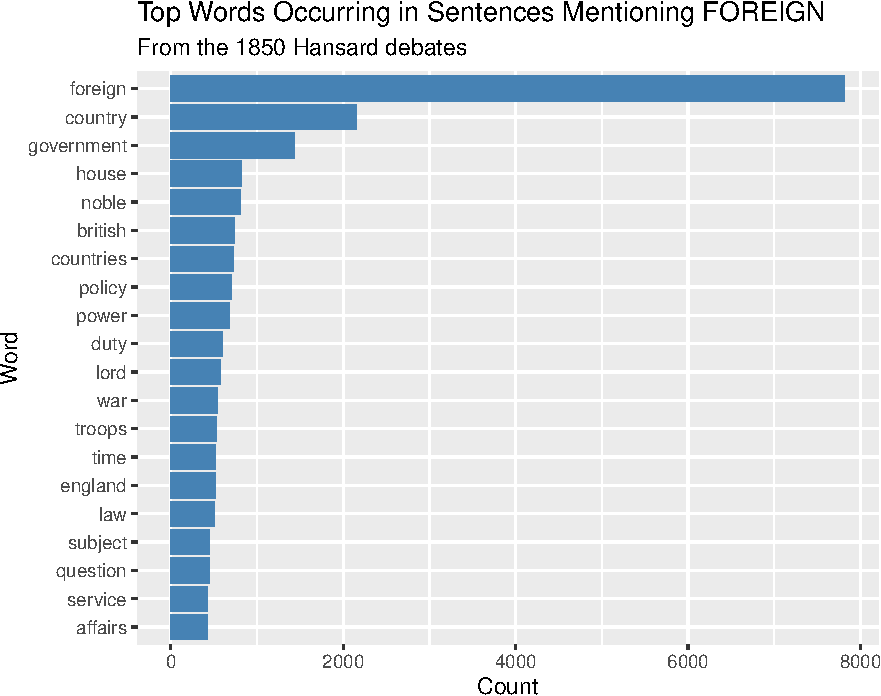
\includegraphics[width=0.8\linewidth]{ch1-11.25.2024_files/figure-latex/generate_plot_foreign-1} \caption{Top words in sentences mentioning foreign (Hansard, 1850)}\label{fig:generate_plot_foreign}
\end{figure}

\begin{figure}
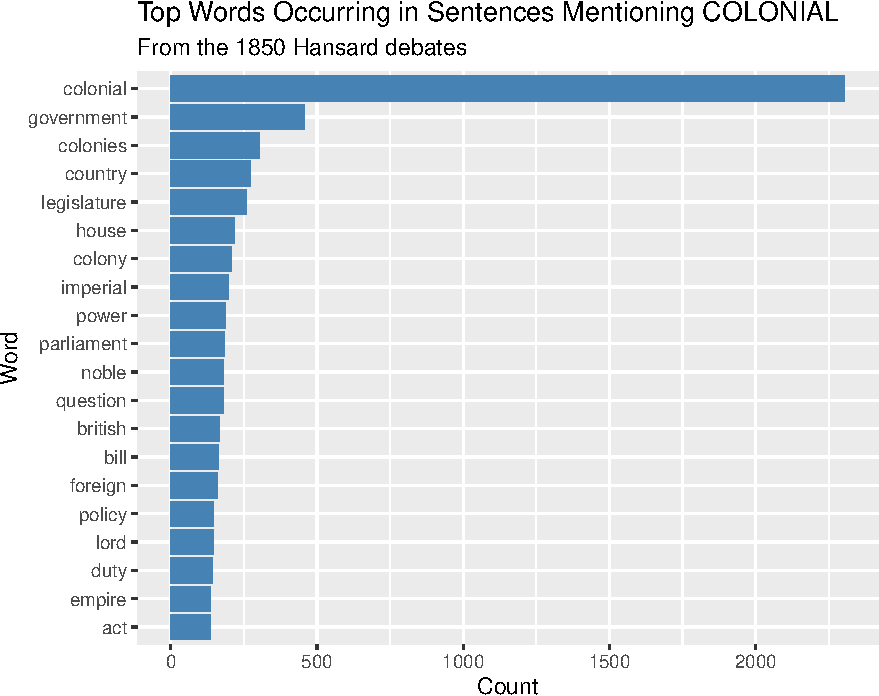
\includegraphics[width=0.8\linewidth]{ch1-11.25.2024_files/figure-latex/generate_plot_colonial-1} \caption{Top words in sentences mentioning colonial (Hansard, 1850)}\label{fig:generate_plot_colonial}
\end{figure}

\begin{figure}
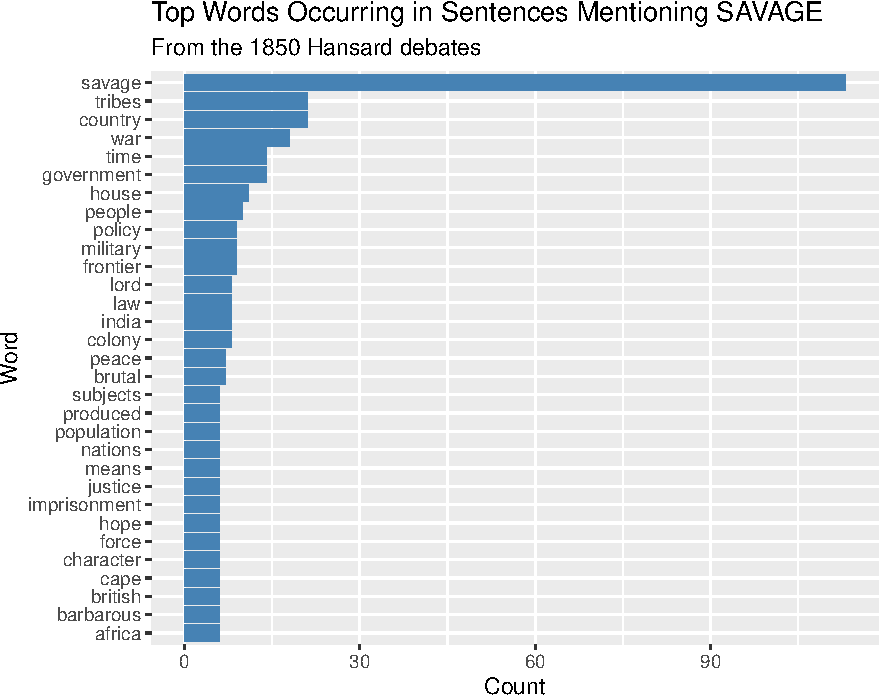
\includegraphics[width=0.8\linewidth]{ch1-11.25.2024_files/figure-latex/generate_plot_savage-1} \caption{Top words in sentences mentioning savage (Hansard, 1850)}\label{fig:generate_plot_savage}
\end{figure}

\begin{figure}
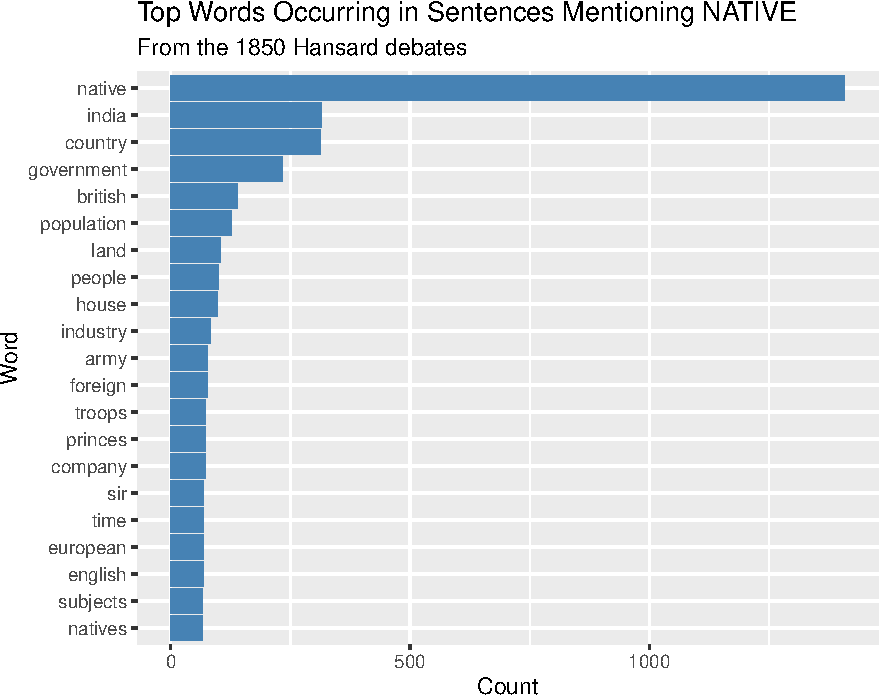
\includegraphics[width=0.8\linewidth]{ch1-11.25.2024_files/figure-latex/generate_plot_native-1} \caption{Top words in sentences mentioning native (Hansard, 1850)}\label{fig:generate_plot_native}
\end{figure}

\begin{figure}
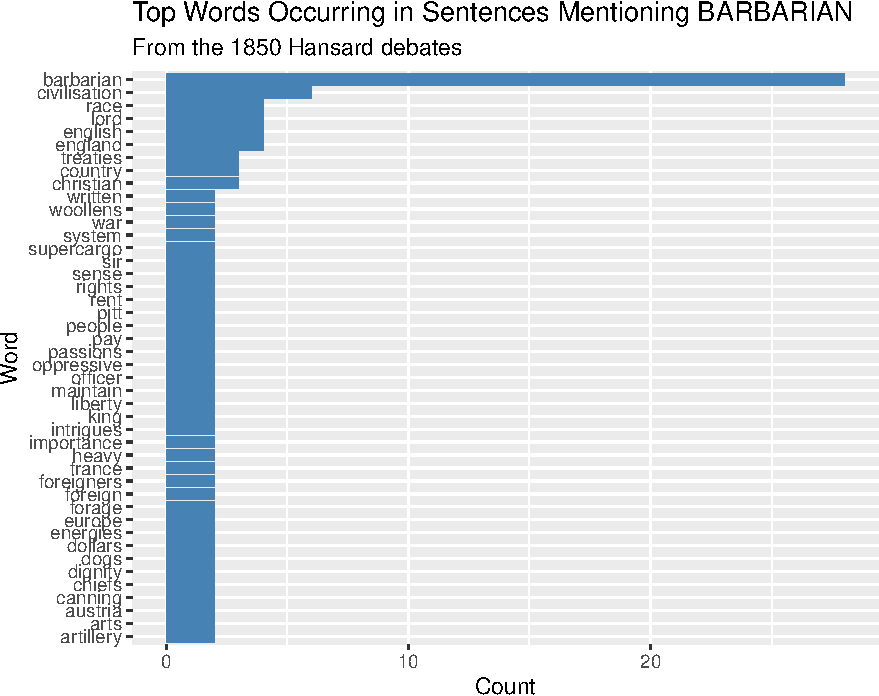
\includegraphics[width=0.8\linewidth]{ch1-11.25.2024_files/figure-latex/generate_plot_barbarian-1} \caption{Top words in sentences mentioning barbarian (Hansard, 1850)}\label{fig:generate_plot_barbarian}
\end{figure}

Producing many graphs in succession (as demonstrated by Figures 1.3 to
1.7) can be useful for exploratory data analysis. Performing a
comparative analysis of graphs side-by-side is one of the main skills
digital humanists use when considering the subtle structures of meaning
and difference that define cultural and political conversations. A
careful comparison between the charts above offers the beginnings of a
nuanced analysis of overlapping terms used by British members of
parliament to refer to people and forces from beyond Britain.

In the results, we see several closely related terms which compose a
field of interrelated meanings. Together, these terms sketch out the
diversity of contrasting ways that British members of parliament spoke
about the world outside of Britain. Some of the attributes ascribed to
the foreign were neutral in value -- for instance, the ``foreign'' was
mainly spoken about in terms of ``laws'', ``duties'', ``trade'', and
``protection'', a world in which different nations ``competed,'' but
generally not a space of moral inferiority and superiority. By contrast,
terms such as ``savage'' and ``barbarian'' telegraphed intellectual and
ethical judgments (for instance, ``brutal'') onto cultures outside of
Britain, typically associating inferiority with racial identity (Metcalf
1995, Colley 1992, Said 1987).

With these terms, a set of binaries is set up by the speakers of
Parliament, dividing the world into ``barbarian'' cultures and
``christian'' ``civilisations,'' a distinction that may have been
analyzed in terms of ``rights,'' ``treaties,'' ``war,'' ``rents,''
``passions,'' ``liberty,'' and ``energies. The distinctions between
the''foreign'' and the ``barbarian'' are invoked in relationship to the
same abstractions we saw typifying the ``foreign,'' including ``law,''
the ``country,'' and ``treaties.'' We also see the ``barbarian'' being
invoked in discussions of many commodities, including ``woolens,''
``forage,'' and ``rent.'' Indeed, the frequent invocation of law,
rights, and foreignness alongside discussions of the barbarian and the
savage suggests that the judgments ascribed to race actually bled into
conversations about law, tariffs, trade, and protectionism, perhaps as
justification for invoking British superiority.

Some readers may assume that we are performing contemporary prejudices
about racism, but the point of this exercise is that it is grounded in a
detailed and careful examination of the words counted by computational
methods. The paragraph above is not concocted out of thin air; it is an
objective description of the prejudices on display in a quantitative
reading of how British members of parliament spoke about the world
beyond their nation. We emphasize that this analysis of the related
language of the ``foreign'' and the ``barbarian'' is not concocted on
the basis of our readings of contemporary theories about racism, but is
actually derived from a careful reading of the language of Hansard, as
well as immersion in writing about the history of empire.

In general, descriptions of arguments made on the basis of word counts
tend to be more persuasive when they take on every word in a list.
Critical thinking about the meaning of proximate keywords is enhanced
when the analyst slows down, taking the trouble to examine the
distinctiveness of each individual keyword and its context. In a further
analysis, the scholar might ask questions that require examining the
results in more detail. They might ask: What biases does each term
convey? Where do the terms overlap? What new information is encapsulated
by some words but not others? We could continue this line of inquiry to
trace the keyword-context pairs back to their original context in
sentences and speeches on the page, showing how speakers used these
words to formulate actual arguments with consequences for the
development of nations and their economies.

Examining collocates provides the basis for critical thinking about the
changing and overlapping meaning of shared concepts in the human past.
Skillful analysts can use approaches of this kind to examine the meaning
of language about categories beyond those of gender, race, nationality,
and commodities, asking questions about the intellectual categories that
governed how members of parliament understood governance itself,
economics, truth, science, virtue, economics, and reason itself. In
every case, the approach would be the same: to examine not merely one or
two keywords, but many related keywords, drawing attention to the subtle
overlap and differences between the terms in usage, and how those
overlapping concepts together work to produce a field of meaning.

\subsection{Critical Thinking About Data and its
Limits}\label{critical-thinking-about-data-and-its-limits}

Another fruitful avenue for critical thinking is the question of which
problems are suited to textual analysis and which are not. Skillful
analysts are wary of asking the wrong question with the wrong tool.
Among the techniques that we have learned in this chapter is the ability
to load and inspect data. Inspecting the data allows the analyst to
notice issues caused by computational processing of text that may cause
issues down the line unless the analyst is aware of them.

Looking at the first lines of \texttt{hansard\_1850}, you might ask
yourself these questions: are all of the lines in the ``text'' field
actually sentences? Are all the words in the same style with respect to
capitalization? We can inspect this further.

Analyzing the entire data frame to further inspect the data can be
distracting since a data frame usually contains multiple columns, some
which may be irrelevant to our current query.

\begin{tabular}{l>{\raggedright\arraybackslash}p{4cm}ll}
\toprule
sentence\_id & text & speechdate & debate\\
\midrule
S3V0108P0\_0 & , which had been prorogued successively from the 1st of August to the 9th of October, from thence to the 20th of Nove... & 1850-01-31 & MEETING OF PARLIAMENT.\\
S3V0108P0\_1 & The Parliament was opened by Commission, the LORDS COMMISSIONERS present being the LORD CHANCELLOR; the LORD PRESIDEN... & 1850-01-31 & MEETING OF PARLIAMENT.\\
S3V0108P0\_2 & called attention to a great omission of their duty on the part of Ministers, with respect to the privileges of their ... & 1850-01-31 & SCOTCH REPRESENTATIVE PEERS.\\
S3V0108P0\_3 & At pre-sent there were two vacancies in the representative Peers of Scotland, in consequence of the deaths of the Ear... & 1850-01-31 & SCOTCH REPRESENTATIVE PEERS.\\
S3V0108P0\_4 & Although the Act of Parliament directed that the proclamation should issue forthwith for the election of representati... & 1850-01-31 & SCOTCH REPRESENTATIVE PEERS.\\
\addlinespace
S3V0108P0\_5 & The Peerage of Scotland was not therefore represented in Parliament at present as it ought to be. & 1850-01-31 & SCOTCH REPRESENTATIVE PEERS.\\
\bottomrule
\end{tabular}

We can make the data more readable by displaying just the data from the
column of interest.

In the following code, we use \texttt{hansard\_1850{[}1:10,\ 2{]}} to
select a specific item from \texttt{hansard\_1850}.
\texttt{hansard\_1850} refers to a data frame or matrix, and
\texttt{{[}1,\ 2{]}} refers to the row and column indices we wish to
look at. The structure of the syntax is this:
\texttt{{[}row,\ column{]}}. The numeric range, \texttt{1:10}, in the
``row'' field tells R to display rows 1 to 10. We put ``2'' in the
``column'' field to tell R to display just the second column, which in
this case is the column containing text.

\begin{longtable}[]{@{}
  >{\raggedright\arraybackslash}p{(\linewidth - 0\tabcolsep) * \real{1.0000}}@{}}
\toprule\noalign{}
\begin{minipage}[b]{\linewidth}\raggedright
x
\end{minipage} \\
\midrule\noalign{}
\endhead
\bottomrule\noalign{}
\endlastfoot
, which had been prorogued successively from the 1st of August to the
9th of October, from thence to the 20th of November, thence to the 16th
of January, and from thence to the 31st January, met this day for
despatch of business. \\
The Parliament was opened by Commission, the LORDS COMMISSIONERS present
being the LORD CHANCELLOR; the LORD PRESIDENT OF THE COUNCIL (the
Marquess of Lansdowne); the LORD PRIVY SEAL (the Earl of Minto); the
LORD CHAMBERLAIN OF THE HOUSEHOLD (the Marquess of Breadalbane); and the
LORD BISHOP OF LONDON. \\
called attention to a great omission of their duty on the part of
Ministers, with respect to the privileges of their Lordships, which
might and ought to have been avoided. \\
At pre-sent there were two vacancies in the representative Peers of
Scotland, in consequence of the deaths of the Earl of Airlie and of Lord
Colville. \\
Although the Act of Parliament directed that the proclamation should
issue forthwith for the election of representative Peers to fill up any
vacancies which might occur, by death or otherwise, no such proclamation
had yet taken place in the case of the two vacancies he had just
mentioned, and the consequence was, that for twenty-four days after the
meeting of Parliament it was not possible for any Scotch representative
Peers to be elected. \\
The Peerage of Scotland was not therefore represented in Parliament at
present as it ought to be. \\
He wanted to know what his noble Friend the President of the Council had
to urge in defence of this omission; for certain it was that the Act of
Parliament had not been obeyed? \\
said, that the Government were not to blame for the omission, as they
had not received any requisition from the usual quarter; they had
strictly followed the previous usage. \\
said, the explanation of the noble Marquess was unsatisfactory. \\
The clause in 5 \& 6 Anne, c.~8, directed what should be done in the
case of vacancies by death, and the words could not well be
misunderstood. \\
\end{longtable}

Some of the rows in the ``text'' field appear not to be complete
sentences. We can investigate this oddity further.

\begin{longtable}[]{@{}
  >{\raggedright\arraybackslash}p{(\linewidth - 0\tabcolsep) * \real{1.0000}}@{}}
\toprule\noalign{}
\begin{minipage}[b]{\linewidth}\raggedright
x
\end{minipage} \\
\midrule\noalign{}
\endhead
\bottomrule\noalign{}
\endlastfoot
, which had been prorogued successively from the 1st of August to the
9th of October, from thence to the 20th of November, thence to the 16th
of January, and from thence to the 31st January, met this day for
despatch of business. \\
\end{longtable}

At this point the dataset is too broad to clearly display by printing,
and some data is cut off. To view the whole text, double-click on the
cell, copy and paste the text into a word processor. The content reads
like so:

\begin{quote}
``, which had been prorogued successively from the 1st of August to the
9th of October, from thence to the 20th of November, thence to the 16th
of January, and from thence to the 31st January, met this day for
despatch {[}sic{]} of business.''
\end{quote}

The first row appears to be a description of the opening of parliament.
Technically, it is a commentary by the printer, not a line of debate.
The convention of discussing parliament's timetables was in place in
1850, but we do not know if the printer always printed this line through
the entire century. We should be aware of this convention and curious
about it if we find ourselves counting months or discussions of words
such as ``business.''

Let's keep inspecting the data, this time turning to the third row in
our dataset.

\begin{longtable}[]{@{}
  >{\raggedright\arraybackslash}p{(\linewidth - 0\tabcolsep) * \real{1.0000}}@{}}
\toprule\noalign{}
\begin{minipage}[b]{\linewidth}\raggedright
x
\end{minipage} \\
\midrule\noalign{}
\endhead
\bottomrule\noalign{}
\endlastfoot
called attention to a great omission of their duty on the part of
Ministers, with respect to the privileges of their Lordships, which
might and ought to have been avoided. \\
\end{longtable}

Here, we see another sentence fragment:

\begin{quote}
``called attention to a great omission of their duty on the part of
Ministers, with respect to the privileges of their Lordships, which
might and ought to have been avoided.''
\end{quote}

The sentence fragment has resulted from attempting to process data while
working on another convention of printing: the fact that the publisher
of Hansard for much of the century gave the name of the speaker followed
by a description of the airing of the speech. On the page, we would be
given the name of a speaker or their title, for example, ``The Lord
Chancellor'' or ``Mr.~Gladstone.'' The passage of text would therefore
read, {[}the speaker{]} ``called attention to a great omission\ldots{}''
-- in other words, it would not be a sentence fragment, so much as a
journalistic description of a speaker. The actual speech probably began
with a statement something like this: ``It is a great omission of their
duty on the part of Ministers{[}\ldots{]}.'' In other words, we are
looking at an oddity that resulted from a mismatch between the
19th-century printed record and how the computer processed the data. We
compiled the data and separate all of the speaker names into one
``field'' of data, which we stored in a separate dataset, to be accessed
in Chapter 2. We have sorted all of the text into the ``text'' field,
which is held in \texttt{hansard\_1850}. The computer did not process
the journalistic description of a speech rather than a normal speech.

Looking at the data presents an opportunity for critical thinking.
Analysts of text as data routinely need to inspect their data and make
sure that the data's quality and density are sufficient to support
claims that they might make.

Already, we can see that the data has certain features that might
interfere with certain kinds of queries, and we should already be
thinking about what these limits might be. Yet the convention of
journalistic reporting on speeches can cause trouble for the analyst if
the analysts are not aware of what has changed. The conventions of
describing speeches changed over the course of the century; at the
beginning of the century, journalistic descriptions were more common.
Later in the century, the conventions changed, and many more speeches
were reported near verbatim without journalistic commentary. We should
be aware of conventions of this kind if we count words which may be
related to journalistic observations such as ``attention,'' ``spoke,''
``declared,'' and so on. Otherwise we may be tempted to interpret
changes to the publisher's conventions of printing speeches as evidence
for changing ideas about politics.

Whether or not data quality will interfere with our ability to make
inferences from the data depends on what we are asking. If we are
counting mentions of the word ``duty'' or the rest of the words in the
content of the speech, then our counts of the words will be correct. If
we contrive to study the history of journalistic observation by tracking
sentence fragments in the dataset, this data will support such a
reading. But we should be wary making inferences about any kind of
inquiry where there is a risk of overlap between substantive discussions
and journalistic observation.

\section{\texorpdfstring{\textbf{\emph{Exercises}}}{Exercises}}\label{exercises}

Expand your grasp of the code and your powers of critical reflection by
trying the following exercises:

\subsection{1) Alter the code above to compare the context for the
keywords ``girl'' and ``woman.'' Do you expect the context to be similar
for both? Does anything surprise you about the
results?}\label{alter-the-code-above-to-compare-the-context-for-the-keywords-girl-and-woman.-do-you-expect-the-context-to-be-similar-for-both-does-anything-surprise-you-about-the-results}

\begin{verbatim}
##       word   n
## 1  husband 237
## 2      law 181
## 3  married 163
## 4 marriage 154
## 5     wife 145
## 6 adultery 143
\end{verbatim}

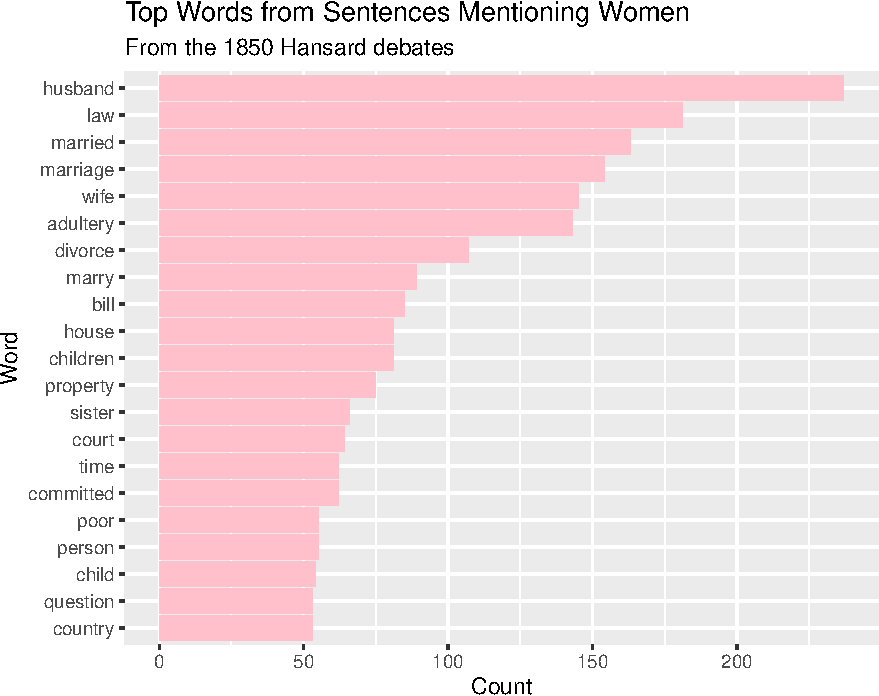
\includegraphics[width=0.8\linewidth]{ch1-11.25.2024_files/figure-latex/find_woman_context-1}

\begin{verbatim}
##     word  n
## 1    age 12
## 2    boy 11
## 3 church  8
## 4   poor  8
## 5   time  8
## 6    law  6
\end{verbatim}

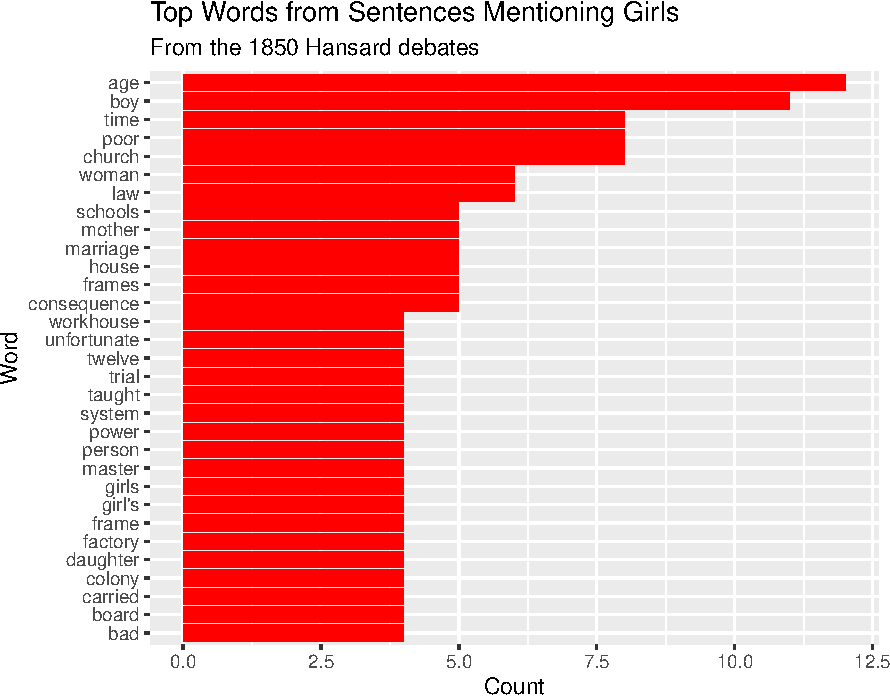
\includegraphics[width=0.8\linewidth]{ch1-11.25.2024_files/figure-latex/find_girl_context-1}

\paragraph{I expected overlap because both words refer to women and
girls, but there is a more significant difference in keywords for girl
and woman than I thought. ``Woman'' in general appears much more
frequently than girl, and is mentioned more in the context of adult
status, legal status, and marriage, with top words like ``husband'' and
``wife.'' This suggested that women was often discussed through their
relationships to men and and within family
roles.}\label{i-expected-overlap-because-both-words-refer-to-women-and-girls-but-there-is-a-more-significant-difference-in-keywords-for-girl-and-woman-than-i-thought.-woman-in-general-appears-much-more-frequently-than-girl-and-is-mentioned-more-in-the-context-of-adult-status-legal-status-and-marriage-with-top-words-like-husband-and-wife.-this-suggested-that-women-was-often-discussed-through-their-relationships-to-men-and-and-within-family-roles.}

\paragraph{Meanwhile ``Girl'' leans into two rather different contexts.
As expected, we see words related to childhood such as ``boy'' and
``schools'' But I was surprised to see ``girl'' also mentioned more in
work context, like with ``workhouse'' and ``factory.'' This sadly
implies that girls were not just seen and discussed as children, but
were subject to child labor and often discussed in relation to it. I was
most surprised to see the words ``unfortunate'' and ``consequence'' pop
up in the context of ``girl'', which implies that girls were likely
framed as victims as
explotation.}\label{meanwhile-girl-leans-into-two-rather-different-contexts.-as-expected-we-see-words-related-to-childhood-such-as-boy-and-schools-but-i-was-surprised-to-see-girl-also-mentioned-more-in-work-context-like-with-workhouse-and-factory.-this-sadly-implies-that-girls-were-not-just-seen-and-discussed-as-children-but-were-subject-to-child-labor-and-often-discussed-in-relation-to-it.-i-was-most-surprised-to-see-the-words-unfortunate-and-consequence-pop-up-in-the-context-of-girl-which-implies-that-girls-were-likely-framed-as-victims-as-explotation.}

\section{2) Use your powers of inspecting data to move from the keyword
context back to the individual sentences. Cut and paste twenty sentences
from the context of each keyword into a word processor. What do you
learn from these sentences that you did not learn from counting
keywords? Does your analysis become more persuasive when quantitative
graphs are accompanied with readings of particular speeches where the
words are examined in their original
context?}\label{use-your-powers-of-inspecting-data-to-move-from-the-keyword-context-back-to-the-individual-sentences.-cut-and-paste-twenty-sentences-from-the-context-of-each-keyword-into-a-word-processor.-what-do-you-learn-from-these-sentences-that-you-did-not-learn-from-counting-keywords-does-your-analysis-become-more-persuasive-when-quantitative-graphs-are-accompanied-with-readings-of-particular-speeches-where-the-words-are-examined-in-their-original-context}

\begin{longtable}[t]{ll}
\caption{\label{tab:woman_sentences_table}Twenty Full Sentences Containing 'Woman'}\\
\toprule
doc\_id & text\\
\midrule
doc1495 & One innocent young woman, who resisted his proposals, and
complained of his conduct to the captain, was taken upon
deck, and buckets of water were thrown upon her.\\
doc1501 & Now, after the publication of such a statement as that of
which he had given their Lordships the substance, was it
likely that any virtuous and well-conducted woman would
trust herself on board of a vessel if she was not sure of
protection?\\
doc2121 & An old woman of seventy was murdered, and the scull of an
idiot was beaten in with the butts of their muskets. ""\\
doc2123 & My noble Friend seems to doubt this; but Mr. Janns,
sub-inspector of police, stales, in his evidence, that the
scull of the unfortunate Sweeny was beaten in with the butts
of their muskets, and that corresponds with the account
given before the coroner, Mr. Berwick goes on to say—
""Another old woman was severely beaten in her house; while
another, who was subsequently saved by the police, was much
injured, and left in her house, which had been set on fire.\\
doc3384 & I fully concur in the sentiment that Her late Majesty had
justly endeared Herself to this country by Her piety, her
charities, and Her exemplary virtues, and that Her name will
be long held in grateful remembrance by every man, woman,
and child in this kingdom.\\
\addlinespace
doc5135 & There is not a man, woman, or child who has not an interest
in the question; and if you were to put on a duty which you
would say would raise the price of corn one shilling, or
eighteenpence, or two shillings the bushel, every man would
count the shilling, or eighteenpence, or two shillings of
wheat which he would have to pay for the support of his
family in addition to that which he pays at the present day.\\
doc8799 & but I, a woman, a wife, a mother, in my own native town,
before the people, who were accustomed to treat me with
respect, was dragged into a square of soldiers, and there I
was scourged with rods, ""\\
doc11026 & But then the clause went on to enact as follows:— ""And when
the opinion of the court is desired in any matter in which
any infant, idiot, lunatic, married woman, or any person
uncertain, unknown, or not to be found, is interested, it
shall be lawful for the Master of the court in rotation to
direct the presenting of such petition by way of special
case, on behalf of the infant, idiot, lunatic, married
woman, or such other person, and such direction of the
Master shall be conclusive to all intents and purposes. ""\\
doc18763 & Now, the Emigration Commissioners were so satisfied of the
danger and difficulty of sending out single women, that it
had long been their practice to discourage their going; nor
would they allow a single woman to embark on board one of
their vessels unless she had some one with her who could
protect her, except in the case of vessels chartered for
such persons as those from the Irish workhouses; and the
abuses that took place there were through the scandalous
fraud sanctioned by the Irish board of guardians, with whose
direct cognisance the master of the work-house substituted
some improper characters to answer to the names of those who
were to have\\
doc20595 & He had also cohabited with the wife of another passenger
(recently married) and with other women, and at Nelson he
left the ship, and continued to live in open adultery with
the married woman. ""\\
\addlinespace
doc22929 & Even to this day we found in the Asiatic nations that
wherever the law regulating the intercourse between man and
woman was of a low description, the morals of the people
were proportionately low.\\
doc26889 & A lieutenant-general in the Army had married a lady, and
then married her aunt; he then married another woman, and
afterwards her niece (the niece of the third wife).\\
doc26961 & No one would deny that second marriages were permitted; but
before a first marriage, a man had ample time to see which
member of a family of sisters was best suited to him, and he
knew that if he lost her the whole world was open before him
to choose any woman, except her sister, to supply her place.\\
doc27054 & There was all the gentleness of woman, with all her
kindliness, all the emotions which could be introduced into
the relationship, without any of the sensual feelings by
which the highest feelings of affection between the sexes
were tarnished.\\
doc27061 & At the time of his marriage, he felt perfect safety against
any mishaps arising from the connection; at the time he
married he loved the woman whom he made his wife; he was now
made a member of a family, with, say, three other sisters,
young and perhaps beautiful, loving him because of the
connection which subsisted between their sister and himself.\\
\addlinespace
doc27262 & He had explained the reasons why the people of this country
regarded marriage with a sister-in-law in a not unfavourable
light; but it had been asked why the friends of the Bill
did not advocate the marriage of a woman with two brothers
in succession, or the marriage of an uncle with his wife's
niece?\\
doc27287 & He could conceive no point of more importance, especially to
women, than an unreserved intimacy between a married woman
and her unmarried sister.\\
doc27295 & There was no case in which a woman would more require the
solace and society of an unmarried sister than when her own
health was failing.\\
doc27297 & He could not but apprehend, also, that if this Bill were to
pass, a married woman might, either from a mistaken regard
for her husband, or out of affection for her children, exact
in some cases a promise on her death-bed from her husband,
that he would marry her sister, even when there was no
affection between the parties.\\
doc27374 & He did not believe that a young unmarried woman could live
in a house with a young widower where there were no ties of
blood to revolt against any feeling of attachment, without
being open to a certain amount of observation.\\
\bottomrule
\end{longtable}

\begin{longtable}[t]{ll}
\caption{\label{tab:girl_sentences_table}Twenty Full Sentences Containing 'Girl'}\\
\toprule
doc\_id & text\\
\midrule
doc2120 & Mr. Fitzmaurice stopped a man in the act of firing at a girl
who was rushing from her father's house.\\
doc18712 & Among these girl"" were twelve girls from a foundling
institution in Dublin, one of whom, a very interesting
girl too, was seduced by the chief officer, and died in
consequence of miscarriage before she could be landed from
the vessel.\\
doc20594 & The first mate of the had seduced and got with child a girl
scarcely 15 years of age, a daughter of a cabin passenger.\\
doc21161 & At all events, the girl lost her life.\\
doc21164 & Under the seventh charge it was alleged that the captain
had failed to prevent unrestricted intercourse between the
officers and sailors and the females on board; that he had
taken one girl to wait upon himself, and that she had died
from the effects of miscarriage before the arrival of the
ship at her destinat\\
\addlinespace
doc21165 & Another girl was named who had been debauched during the
voyage, and who was then an inmate of a notorious brothel
in the colony; and another, who also had waited upon the
captain, had been seen in a situation which left no doubt
that she also was receiving the wages of prostitution.\\
doc21167 & Now, he wanted to know had any inquiry taken place into the
death of the unfortunate orphan girl?\\
doc21659 & In the National schools in London and the neighbourhood,
there were three boys educated to two girls; but in the
British and Foreign schools in the metropolis and its
neighbourhood, there was only one girl to two boys.\\
doc33352 & One girl who lived at no great distance from the factory
stated that she went home again, and got into bed until she
was wanted again at the factory.\\
doc33353 & Another girl, who walked some miles to her work, said she
was obliged to spend her time in an eating-house until her
hour for resuming work in the factory arrived.\\
\addlinespace
doc39260 & Two persons were there charged with causing the death of
a young girl whom they had obtained from the neighbouring
workhouse at Bideford, in the capacity of a servant.\\
doc39261 & The treatment this unfortunate girl had received, had
excited feelings of indignation and horror in the breast
of every person who had become acquainted with the affair;
but through some informality or legal technicality in the
proceedings, the perpetrators of these horrors had totally
escaped punishment.\\
doc39262 & In the course of the proceedings an allegation was made,
or rather not denied, that the master of the workhouse at
Bideford, Thomas Surnam, bad not only failed to discourage,
but had actually excited and encouraged, these two
monsters to further barbarities, if possible, towards this
unfortunate girl.\\
doc39263 & So much so, that upon one occasion, when the poor girl was
unable to carry a pail in consequence of the barbarities
which had been inflicted upon her, the workhouse master,
when informed of her inability to do so, brutally said, that
""that they ought have broken a stick about her back\\
doc43309 & Member to refer to the inquiry promised by the Poor Law
Board into the conduct of Mr. Surman, the master of the
Bideford union workhouse, with reference to the treatment of
the poor girl whose shocking death had formed the subject of
a late judicial investigation.\\
\addlinespace
doc70529 & The case was inquired into before the board of guardians,
and they decided that they had already voted that the
girl was a Presbyterian, and that the matron was perfectly
justified in dragging her to a Presbyterian\\
doc71314 & Having the concurrence of the legislature of Sydney, be
should like to suggest whether it would not be better at
once to commence a system, which, if carried out, would lead
to a greater demand for boy as well as girl emigrants from
the workhouses of this country.\\
doc75282 & At present a boy or girl under 13 years could be employed
only six and a half hours each day.\\
doc97401 & The marriage of an old man with a young girl, of an old
woman with a youth, of a man who has a family of daughters
with a woman of bad character, and many others; but the law
does not interfere to prevent them.\\
doc98252 & it would be absurd to bring in a Bill to prevent marriage
between a man of 75 and a girl of 16; but was it not quite
clear that there was a great difference between marriages
which were expedient, and marriages which were inces- tuous?\\
\bottomrule
\end{longtable}

\paragraph{Reading the original sentences taught me things the keyword
counts could not; I could see how the terms worked in conjunction with
other words rather than just seeing how often they show up. Creating
separate lists for both ``women'' and ``girls'' makes it clear that
there are vast differences in their contexts. For example, while the
frequency tables suggest that ``woman'' is tied to marriage, legality,
and ``protection,'' the sentences show what that protection actually
means in
debate.}\label{reading-the-original-sentences-taught-me-things-the-keyword-counts-could-not-i-could-see-how-the-terms-worked-in-conjunction-with-other-words-rather-than-just-seeing-how-often-they-show-up.-creating-separate-lists-for-both-women-and-girls-makes-it-clear-that-there-are-vast-differences-in-their-contexts.-for-example-while-the-frequency-tables-suggest-that-woman-is-tied-to-marriage-legality-and-protection-the-sentences-show-what-that-protection-actually-means-in-debate.}

\paragraph{Women are often mentioned in the context of their
relationships with men, often as subjects of unwanted advances, as in
one sentence: ``One innocent young woman, who resisted his proposals,
and complained of his conduct to the captain, was taken upon deck'' or
as weak people unable to defend themselves: ``nor would they allow a
single woman to embark on board one of their vessels unless she had some
one with her who could protect her.'' We also see how gender traits
might have been idealized: ``There was all the gentleness of woman ,
with all her kindliness , all the emotions which could be introduced
into the
relationship''}\label{women-are-often-mentioned-in-the-context-of-their-relationships-with-men-often-as-subjects-of-unwanted-advances-as-in-one-sentence-one-innocent-young-woman-who-resisted-his-proposals-and-complained-of-his-conduct-to-the-captain-was-taken-upon-deck-or-as-weak-people-unable-to-defend-themselves-nor-would-they-allow-a-single-woman-to-embark-on-board-one-of-their-vessels-unless-she-had-some-one-with-her-who-could-protect-her.-we-also-see-how-gender-traits-might-have-been-idealized-there-was-all-the-gentleness-of-woman-with-all-her-kindliness-all-the-emotions-which-could-be-introduced-into-the-relationship}

\paragraph{With ``girl,'' the lists talked about schools and labor, but
the sentences reveal how often girls were discussed through coercion and
regulation. Surprisingly and rather disturbingly, we see even more
explicit content regarding sexual advances than with women. One sentence
describes the impregnation of a girl: ``The first mate of the {[}ship{]}
had seduced and got with child a girl scarcely 15 years of age, a
daughter of a cabin passenger'' and later discussion of efforts ``to
prevent unrestricted intercourse between the officers and sailors and
the females on board,'' including one man that ``had taken one girl to
wait upon himself, and that she had died from the effects of
miscarriage'' Another sentence discusses the limits for youth labor:
``At present a boy or girl under 13 years could be employed only six and
a half hours each day.'' This comparison reveals that while ``women''
were discussed more as subjects of legal protection, ``girls'' were
often discussed as victims of physical or systemic exploitation, through
labor and
seduction.}\label{with-girl-the-lists-talked-about-schools-and-labor-but-the-sentences-reveal-how-often-girls-were-discussed-through-coercion-and-regulation.-surprisingly-and-rather-disturbingly-we-see-even-more-explicit-content-regarding-sexual-advances-than-with-women.-one-sentence-describes-the-impregnation-of-a-girl-the-first-mate-of-the-ship-had-seduced-and-got-with-child-a-girl-scarcely-15-years-of-age-a-daughter-of-a-cabin-passenger-and-later-discussion-of-efforts-to-prevent-unrestricted-intercourse-between-the-officers-and-sailors-and-the-females-on-board-including-one-man-that-had-taken-one-girl-to-wait-upon-himself-and-that-she-had-died-from-the-effects-of-miscarriage-another-sentence-discusses-the-limits-for-youth-labor-at-present-a-boy-or-girl-under-13-years-could-be-employed-only-six-and-a-half-hours-each-day.-this-comparison-reveals-that-while-women-were-discussed-more-as-subjects-of-legal-protection-girls-were-often-discussed-as-victims-of-physical-or-systemic-exploitation-through-labor-and-seduction.}

\section{\texorpdfstring{3) We have examined `coal' and `corn' in the
1850s. Now, search for the words `coal' and `corn' in dataset
\texttt{hansard\_1820}. Were they being used in the same way? What
changed?}{3) We have examined `coal' and `corn' in the 1850s. Now, search for the words `coal' and `corn' in dataset hansard\_1820. Were they being used in the same way? What changed?}}\label{we-have-examined-coal-and-corn-in-the-1850s.-now-search-for-the-words-coal-and-corn-in-dataset-hansard_1820.-were-they-being-used-in-the-same-way-what-changed}

\begin{verbatim}
##           word    n
## 1        price 1166
## 2      foreign  633
## 3      country  601
## 4         duty  345
## 5         laws  300
## 6        trade  288
## 7  importation  278
## 8       market  255
## 9       prices  225
## 10     measure  210
## 11       house  186
## 12     average  182
## 13    imported  182
## 14    quantity  172
## 15        time  168
\end{verbatim}

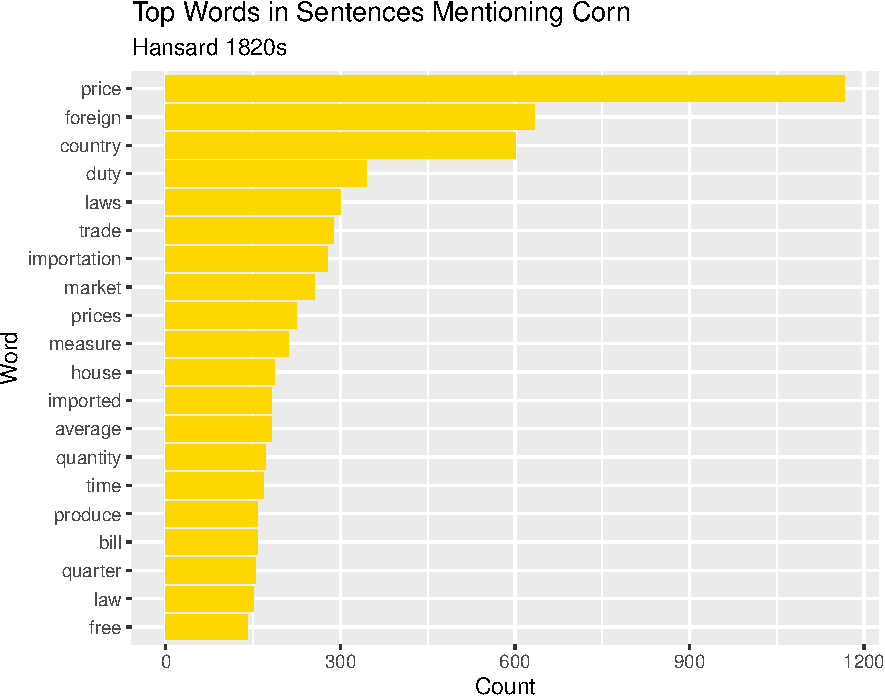
\includegraphics[width=0.8\linewidth]{ch1-11.25.2024_files/figure-latex/corn1820s-1}

\begin{verbatim}
##           word  n
## 1       inland 38
## 2        coals 35
## 3         duty 33
## 4       owners 32
## 5       london 27
## 6       duties 26
## 7        trade 22
## 8          sea 18
## 9          tax 18
## 10       mines 16
## 11      market 15
## 12       north 15
## 13    northern 12
## 14 proprietors 12
## 15      repeal 12
\end{verbatim}

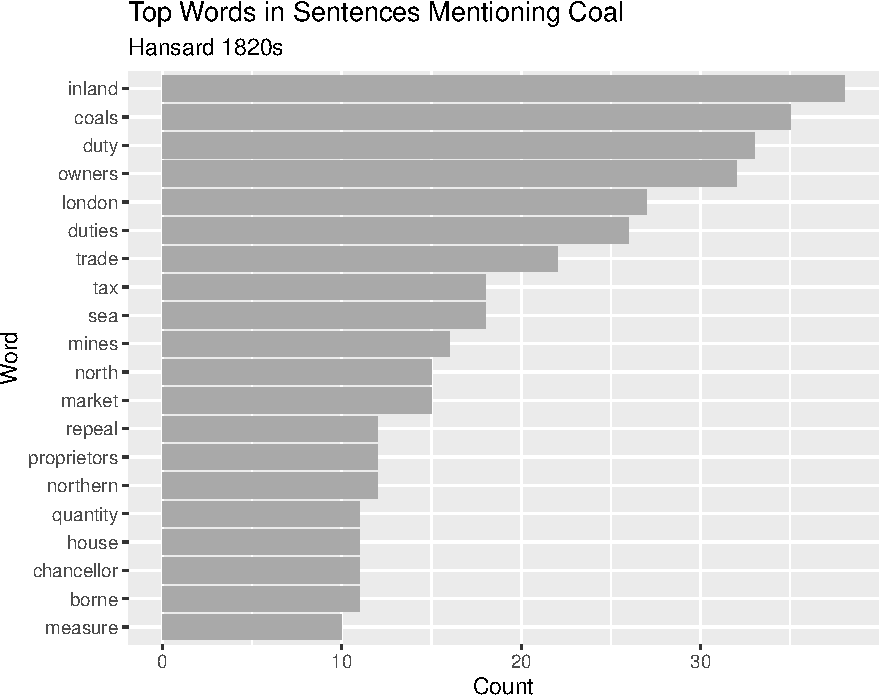
\includegraphics[width=0.8\linewidth]{ch1-11.25.2024_files/figure-latex/coal1820-1}

\paragraph{In the 1820s, we see that''corn'' is strongly associated with
economic regulation and trade policy, with top keywords like ``price,''
``foreign,'' and ``importation.'' This fits the landscape right after
the Corn Laws passed in 1815, which kept prices high to protect domestic
farmers, subsequently causing a lot of economic suffering because it
meant higher food costs for everyone else. In the 1850s as we saw above,
we see a shift to words like ``repeal'' ``free'' ``noble'' after the
corn laws had been repealed in 1846. It makes sense that the 1850s
debates shift in discussion toward free trade, often framing it in a
more positive or settled political light than
before.}\label{in-the-1820s-we-see-thatcorn-is-strongly-associated-with-economic-regulation-and-trade-policy-with-top-keywords-like-price-foreign-and-importation.-this-fits-the-landscape-right-after-the-corn-laws-passed-in-1815-which-kept-prices-high-to-protect-domestic-farmers-subsequently-causing-a-lot-of-economic-suffering-because-it-meant-higher-food-costs-for-everyone-else.-in-the-1850s-as-we-saw-above-we-see-a-shift-to-words-like-repeal-free-noble-after-the-corn-laws-had-been-repealed-in-1846.-it-makes-sense-that-the-1850s-debates-shift-in-discussion-toward-free-trade-often-framing-it-in-a-more-positive-or-settled-political-light-than-before.}

\paragraph{For coal in the 1820s, we see more location-centric and
transportation terms like ``inland,'' ``north'' and ``London.'' This
makes sense historically because back before railways became common,
coal was usually transported in large quantities by ship from Northern
regions to London. In the 1850s, we see more industrial terms like
``iron,'' ``steam,'' and ``engine.'' This correlates with how coal had
evolved as an energy source, from heating homes to fueling engines. By
the 1850s, steam power and railways were becoming more prominent and
coal was being used to power steam engines. - making discussions around
it focused on the industrial role it had taken
on.}\label{for-coal-in-the-1820s-we-see-more-location-centric-and-transportation-terms-like-inland-north-and-london.-this-makes-sense-historically-because-back-before-railways-became-common-coal-was-usually-transported-in-large-quantities-by-ship-from-northern-regions-to-london.-in-the-1850s-we-see-more-industrial-terms-like-iron-steam-and-engine.-this-correlates-with-how-coal-had-evolved-as-an-energy-source-from-heating-homes-to-fueling-engines.-by-the-1850s-steam-power-and-railways-were-becoming-more-prominent-and-coal-was-being-used-to-power-steam-engines.---making-discussions-around-it-focused-on-the-industrial-role-it-had-taken-on.}

\section{\texorpdfstring{4) Above, we created the list of words called
\texttt{identifiers\_for\_woman}. Use the operator \texttt{\%in\%} with
the command \texttt{filter()} to create a list of the words in the
context of discussions of women. Create another list called
\texttt{identifiers\_for\_man} and do the same for discussions of men.
Create visualizations for the top terms used in discussions of men and
women.}{4) Above, we created the list of words called identifiers\_for\_woman. Use the operator \%in\% with the command filter() to create a list of the words in the context of discussions of women. Create another list called identifiers\_for\_man and do the same for discussions of men. Create visualizations for the top terms used in discussions of men and women.}}\label{above-we-created-the-list-of-words-called-identifiers_for_woman.-use-the-operator-in-with-the-command-filter-to-create-a-list-of-the-words-in-the-context-of-discussions-of-women.-create-another-list-called-identifiers_for_man-and-do-the-same-for-discussions-of-men.-create-visualizations-for-the-top-terms-used-in-discussions-of-men-and-women.}

\begin{verbatim}
##       word    n
## 1  husband 1192
## 2      law  979
## 3 children  865
## 4 marriage  825
## 5     bill  549
## 6   wife's  529
\end{verbatim}

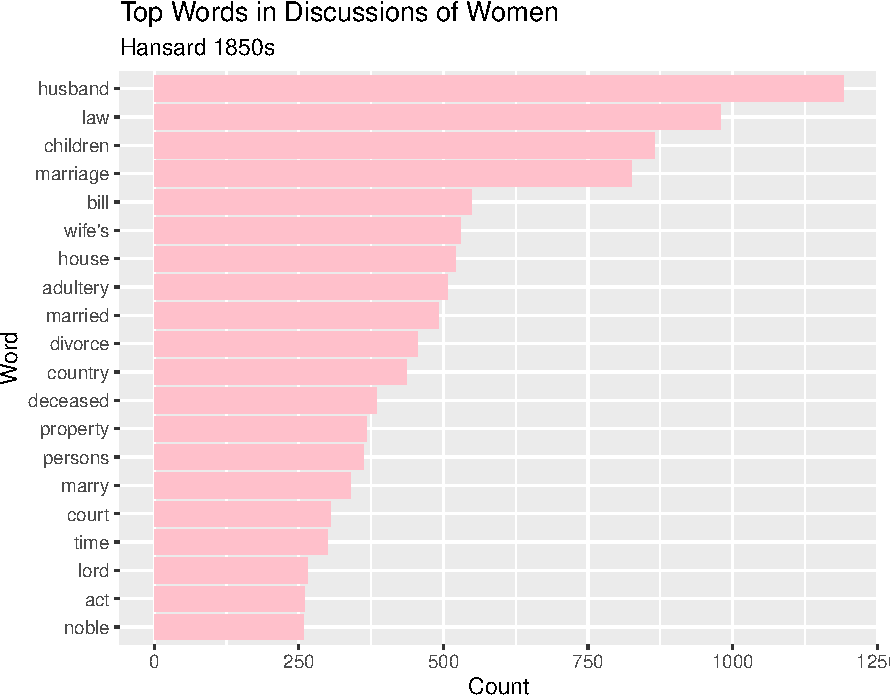
\includegraphics[width=0.8\linewidth]{ch1-11.25.2024_files/figure-latex/women_context-1}

\begin{verbatim}
##            word    n
## 1       husband 1567
## 2        father  918
## 3       brother  891
## 4          boys  600
## 5           boy  315
## 6          male  278
## 7      brothers  219
## 8       fathers  182
## 9      husbands  165
## 10        males   94
## 11        uncle   76
## 12  grandfather   26
## 13 grandfathers   12
## 14       uncles    7
\end{verbatim}

\begin{verbatim}
##         word    n
## 1    country 5360
## 2      house 4874
## 3 government 3990
## 4       lord 3118
## 5       time 2971
## 6      noble 2787
\end{verbatim}

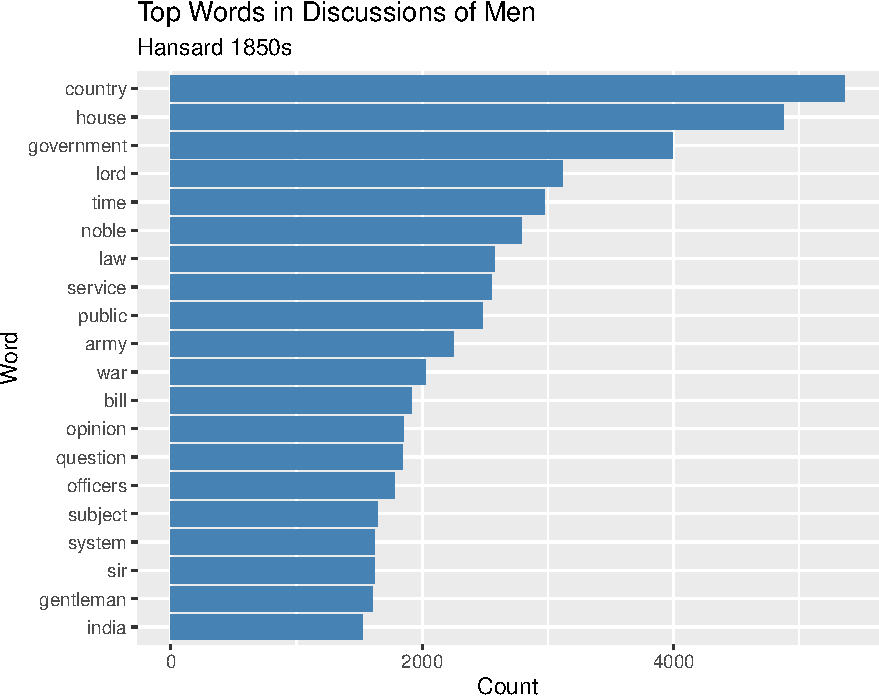
\includegraphics[width=0.8\linewidth]{ch1-11.25.2024_files/figure-latex/man_context-1}

\paragraph{We see that compared to women and girls, men-identifier
sentences skew toward public life and politics, with top context terms
like ``government,'' ``law,'' ``service,'' and ``public.'' This suggests
that men were more often framed as political actors and participants in
state institutions, while women were more often discussed through
domestic roles, dependency, and legal ``protection'' rather than
autonomy.}\label{we-see-that-compared-to-women-and-girls-men-identifier-sentences-skew-toward-public-life-and-politics-with-top-context-terms-like-government-law-service-and-public.-this-suggests-that-men-were-more-often-framed-as-political-actors-and-participants-in-state-institutions-while-women-were-more-often-discussed-through-domestic-roles-dependency-and-legal-protection-rather-than-autonomy.}

\section{5) Reflect on your work so far -- in which you have compared
words for gender, the concept of the foreign, and the context of
discussions of different commodities. You have made comparisons over
time and comparisons of lists. Which of the comparisons do you find the
most productive of insight about how certain words were being used in
political debate? Are you persuaded by large numbers? Are you persuaded
by subtle variations in the context of different words? Write a
paragraph explaining for yourself wherein constitutes the most
persuasive usage of comparisons between keyword in
context.}\label{reflect-on-your-work-so-far-in-which-you-have-compared-words-for-gender-the-concept-of-the-foreign-and-the-context-of-discussions-of-different-commodities.-you-have-made-comparisons-over-time-and-comparisons-of-lists.-which-of-the-comparisons-do-you-find-the-most-productive-of-insight-about-how-certain-words-were-being-used-in-political-debate-are-you-persuaded-by-large-numbers-are-you-persuaded-by-subtle-variations-in-the-context-of-different-words-write-a-paragraph-explaining-for-yourself-wherein-constitutes-the-most-persuasive-usage-of-comparisons-between-keyword-in-context.}

\paragraph{We saw that examining sentence contexts for individual
keywords was more productive than simply counting how many times these
words appeared.The word counts are useful for showing what topics are
most prominent, but the context is what reveals the meaning and
political framing of them. Comparing near-synonyms like ``girl'' vs
``woman'' was especially insightful because it showed that each term
carried different assumptions about age, vulnerability, and social role.
Comparing words across time, like ``corn'' in the 1820s vs the 1850s,
made it clear how historical conditions, laws, and policy debates
reshaped the language surrounding the same entity. Visualizing these
comparisons helps because we can see these patterns and subtle
differences upfront, but the most convincing analysis combines the
graphs with a few representative sentences, showing how the quantitative
results we get are rooted in real
writing.}\label{we-saw-that-examining-sentence-contexts-for-individual-keywords-was-more-productive-than-simply-counting-how-many-times-these-words-appeared.the-word-counts-are-useful-for-showing-what-topics-are-most-prominent-but-the-context-is-what-reveals-the-meaning-and-political-framing-of-them.-comparing-near-synonyms-like-girl-vs-woman-was-especially-insightful-because-it-showed-that-each-term-carried-different-assumptions-about-age-vulnerability-and-social-role.-comparing-words-across-time-like-corn-in-the-1820s-vs-the-1850s-made-it-clear-how-historical-conditions-laws-and-policy-debates-reshaped-the-language-surrounding-the-same-entity.-visualizing-these-comparisons-helps-because-we-can-see-these-patterns-and-subtle-differences-upfront-but-the-most-convincing-analysis-combines-the-graphs-with-a-few-representative-sentences-showing-how-the-quantitative-results-we-get-are-rooted-in-real-writing.}

\section{6) For the visualizations of the terms associated with
different terms for the ``foreign,'' tell us: What biases does each term
convey? Where do the terms overlap? What new information is encapsulated
by some words but not others? What do we learn from this exercise about
the prejudices of Britain's members of parliament in the
1850s?}\label{for-the-visualizations-of-the-terms-associated-with-different-terms-for-the-foreign-tell-us-what-biases-does-each-term-convey-where-do-the-terms-overlap-what-new-information-is-encapsulated-by-some-words-but-not-others-what-do-we-learn-from-this-exercise-about-the-prejudices-of-britains-members-of-parliament-in-the-1850s}

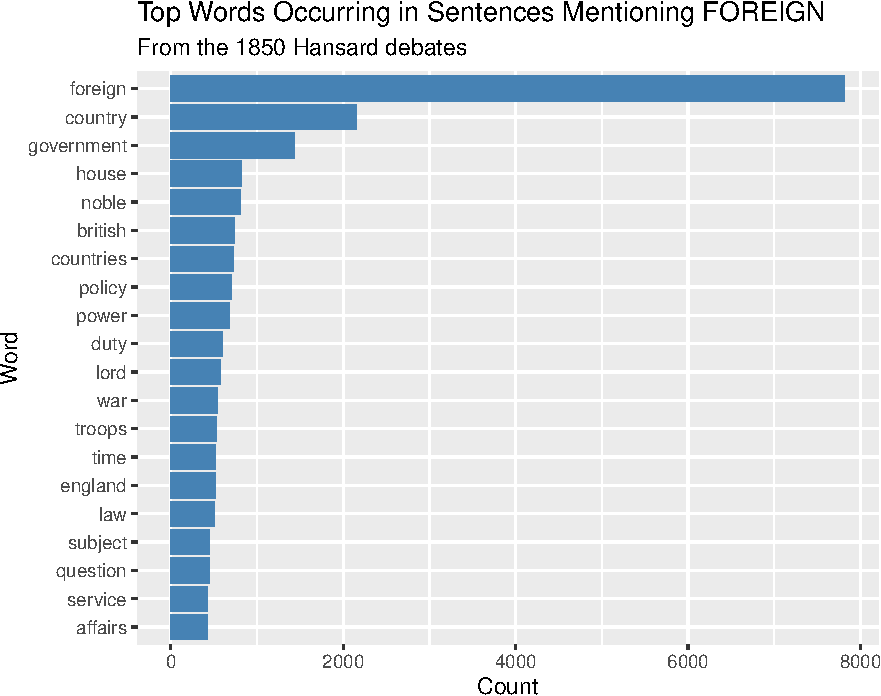
\includegraphics[width=0.8\linewidth]{ch1-11.25.2024_files/figure-latex/word_plots-1}
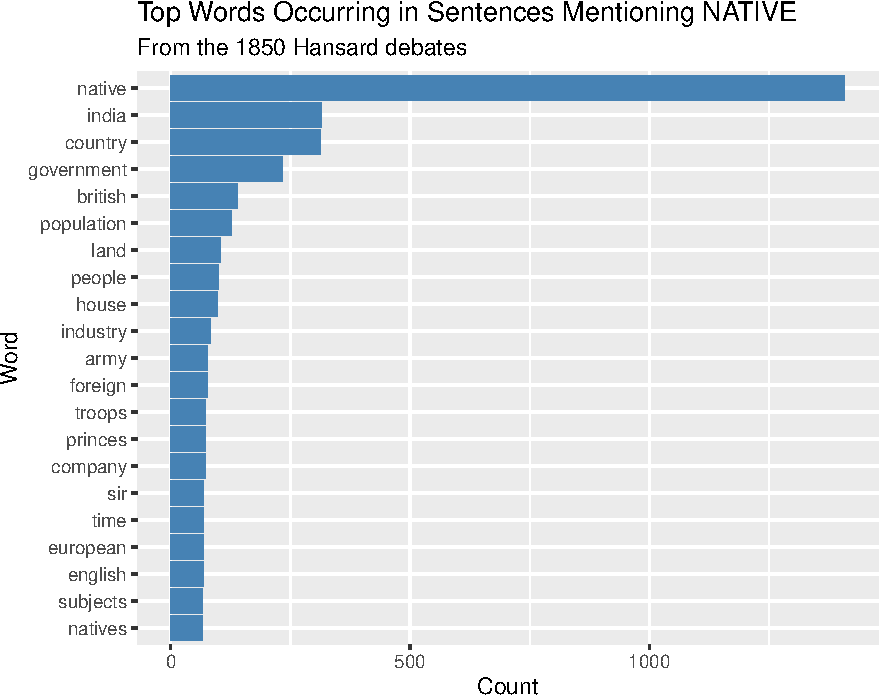
\includegraphics[width=0.8\linewidth]{ch1-11.25.2024_files/figure-latex/word_plots-2}
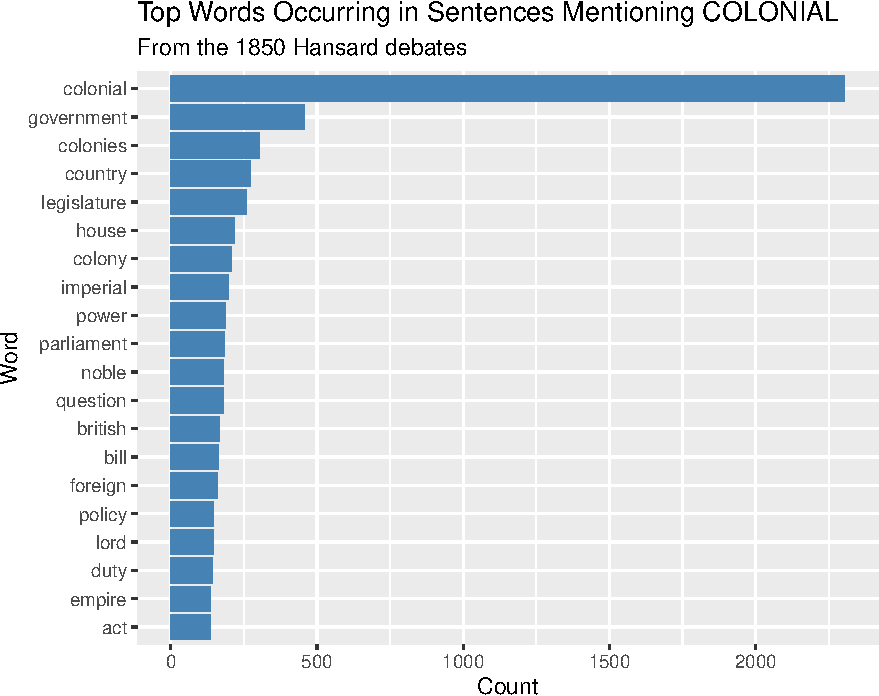
\includegraphics[width=0.8\linewidth]{ch1-11.25.2024_files/figure-latex/word_plots-3}
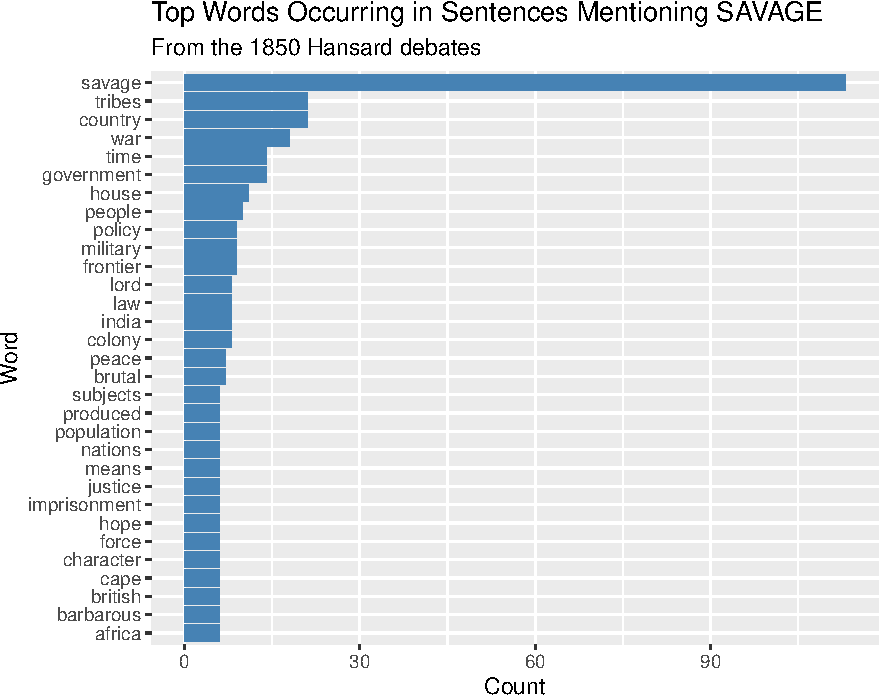
\includegraphics[width=0.8\linewidth]{ch1-11.25.2024_files/figure-latex/word_plots-4}
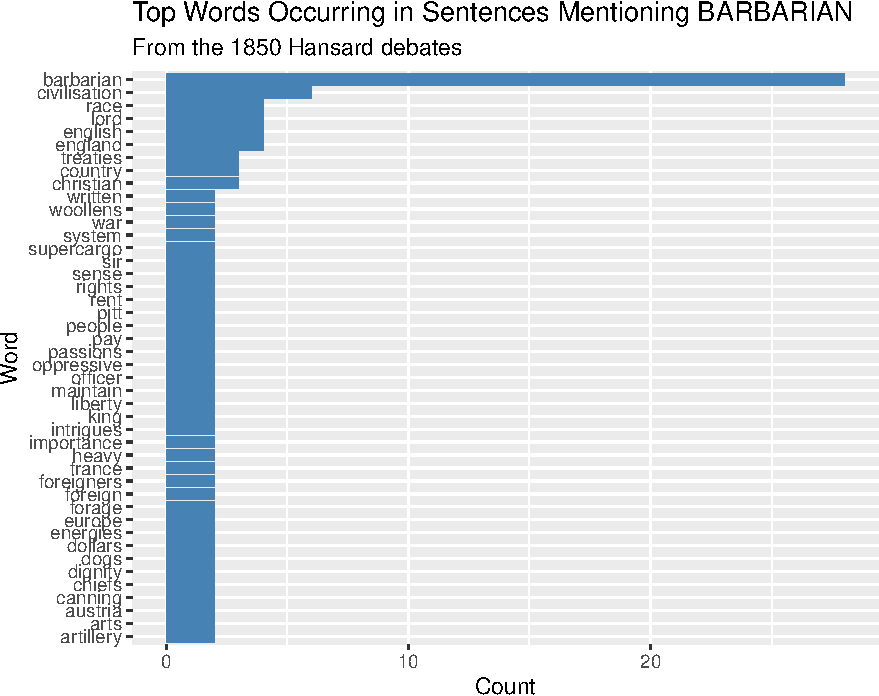
\includegraphics[width=0.8\linewidth]{ch1-11.25.2024_files/figure-latex/word_plots-5}

\paragraph{We can see in the ``foreign'' plot that this term is
relatively neutral, associated with economic and diplomatic terms like
``laws,'' ``duties,'' ``trade,'' and ``policy.'' It frames interaction
as a matter of statecraft rather than
morality.}\label{we-can-see-in-the-foreign-plot-that-this-term-is-relatively-neutral-associated-with-economic-and-diplomatic-terms-like-laws-duties-trade-and-policy.-it-frames-interaction-as-a-matter-of-statecraft-rather-than-morality.}

\paragraph{In comparison, ``savage'' and ``barbarian'' have much
stronger and controversial associations, conveying harsh judgments about
morality and intellect. ``Savage'' is rather dehumanizing and is
associated with violent words like ``brutal,'' ``force,'' and ``war,''
as well as ``tribes,'' ``India,'' and ``Africa.'' This shows that these
terms framed non-British peoples as violent or inferior. Compared to the
other words, ``savage'' shows the strongest biases, depicting minority
groups as less civilized and more threatening. ``Barbarian'' is less
explicit about race, but shows a similar issue as ``savage.'' By
including terms like ``civilization,'' ``Christian,'' and
``oppressive,'' it implies a bias where European standards are the main
measure of legitimacy and
worth.}\label{in-comparison-savage-and-barbarian-have-much-stronger-and-controversial-associations-conveying-harsh-judgments-about-morality-and-intellect.-savage-is-rather-dehumanizing-and-is-associated-with-violent-words-like-brutal-force-and-war-as-well-as-tribes-india-and-africa.-this-shows-that-these-terms-framed-non-british-peoples-as-violent-or-inferior.-compared-to-the-other-words-savage-shows-the-strongest-biases-depicting-minority-groups-as-less-civilized-and-more-threatening.-barbarian-is-less-explicit-about-race-but-shows-a-similar-issue-as-savage.-by-including-terms-like-civilization-christian-and-oppressive-it-implies-a-bias-where-european-standards-are-the-main-measure-of-legitimacy-and-worth.}

\paragraph{``Native'' is dominated by terms like ``India,'' ``British,''
``population,'' ``land,'' and even ``princes.'' This might imply that
natives were often discussed in relation to British colonial rule,
emphasizing the management and control of colonized subjects rather than
just their status as ``foreign'' or their
morality.}\label{native-is-dominated-by-terms-like-india-british-population-land-and-even-princes.-this-might-imply-that-natives-were-often-discussed-in-relation-to-british-colonial-rule-emphasizing-the-management-and-control-of-colonized-subjects-rather-than-just-their-status-as-foreign-or-their-morality.}

\paragraph{Colonial appears more government-centric, with terms like
``colonies,'' ``government,'' ``imperial,'' and ``legislature.'' This
suggests that discussions of the ``colonial'' were more focused on the
administrative side of the empire rather than people or
cultures.}\label{colonial-appears-more-government-centric-with-terms-like-colonies-government-imperial-and-legislature.-this-suggests-that-discussions-of-the-colonial-were-more-focused-on-the-administrative-side-of-the-empire-rather-than-people-or-cultures.}

\paragraph{There is a lot of overlap in these five terms, especially
within the sectors of law and governance, with ``foreign,'' ``country,''
and ``British'' recurring. Looking at the terms all together, we can see
that MPs in the 1850s did not use a singular term for non-British
peoples, but had several labels that carried different connotations,
switching between them depending on the arguments and topics. While
``foreign'' and ``colonial'' were the most ``governmentally neutral,''
``natives'' implied that certain populations needed governing,
while''savage'' and ``barbarian'' framed people as threats to European
civilization, justifying imperial control and racist attitudes. The
consistent use of legal language across all these terms shows that these
racial and cultural biases were not just personal prejudices, but were
built into the frameworks of law and government
itself.}\label{there-is-a-lot-of-overlap-in-these-five-terms-especially-within-the-sectors-of-law-and-governance-with-foreign-country-and-british-recurring.-looking-at-the-terms-all-together-we-can-see-that-mps-in-the-1850s-did-not-use-a-singular-term-for-non-british-peoples-but-had-several-labels-that-carried-different-connotations-switching-between-them-depending-on-the-arguments-and-topics.-while-foreign-and-colonial-were-the-most-governmentally-neutral-natives-implied-that-certain-populations-needed-governing-whilesavage-and-barbarian-framed-people-as-threats-to-european-civilization-justifying-imperial-control-and-racist-attitudes.-the-consistent-use-of-legal-language-across-all-these-terms-shows-that-these-racial-and-cultural-biases-were-not-just-personal-prejudices-but-were-built-into-the-frameworks-of-law-and-government-itself.}

\subsection{AI Use Statement}\label{ai-use-statement}

\emph{I used AI tools in the following ways:}

\emph{\textbf{Tool used:} ChatGPT}

\begin{itemize}
\item
  \emph{\textbf{Purpose:} I used ChatGPT for technical debugging support
  while completing Question 2. My sentence tables were rendering
  incorrectly in the R Markdown file, with several issues like slow
  rendering, clipped phrases, and stray characters appearing in the
  middle of sentences. I asked for help troubleshooting formatting and
  for suggestions to shorten or wrap the table text so the output would
  render properly. I also used it to resolve execution errors ``Quitting
  from ch1-11.25.2024\ldots Execution halted'' that happened in separate
  code chunks.}

  \emph{\textbf{Tasks performed independently by me:} I ran and
  interpreted the Chapter 1 code myself, modified the code to fit the
  assignment questions, selected and reviewed the sentences used for
  close reading, and wrote all summary and reflection responses.}
\end{itemize}

\end{document}
